\chapter{Nonlinear systems} \label{nlin:chapter}

%%%%%%%%%%%%%%%%%%%%%%%%%%%%%%%%%%%%%%%%%%%%%%%%%%%%%%%%%%%%%%%%%%%%%%%%%%%%%%

\section{Linearization, critical points, and equilibria}
\label{linearization:section}

\sectionnotes{1 lecture\EPref{, \S6.1--\S6.2 in \cite{EP}}\BDref{,
\S9.2--\S9.3 in \cite{BD}}}

%\subsection{Nonlinear equations}

Except for a few brief detours in \chapterref{fo:chapter},
we considered mostly linear
equations.  Linear equations suffice in many applications, but in reality
most phenomena require nonlinear equations.  Nonlinear equations, however,
are notoriously more difficult to understand than linear ones, and 
many strange new phenomena appear when we allow our equations to be
nonlinear.

Not to worry, we did not waste all this time studying linear equations.
Nonlinear equations can often be approximated by linear ones if we only need
a solution \myquote{locally,} for example, only for a short period of time, or
only for certain parameters.  Understanding linear equations can
also give us qualitative understanding about a more general nonlinear
problem.  The idea is similar to what you did in calculus in trying to
approximate a function by a line with the right slope.

\begin{mywrapfigsimp}{1.45in}{1.75in}
\noindent
\inputpdft{mv-pend}
\end{mywrapfigsimp}
In \sectionref{sec:mv} we looked at the pendulum of %mass $m$ and
length $L$.  The goal was to solve for the angle $\theta(t)$ as
a function of the time $t$.  The equation for the setup is
the nonlinear equation
\begin{equation*}
\theta'' + \frac{g}{L} \sin \theta = 0 .
\end{equation*}
Instead of solving this equation, we solved the rather easier linear
equation
\begin{equation*}
\theta'' + \frac{g}{L} \theta = 0 .
\end{equation*}
While the solution to the linear equation is not exactly what we were
looking for, it is rather close to the original, as long as the
angle $\theta$ is small and the time period involved is short.

You might ask: Why don't we just solve the nonlinear problem?  Well, it
might be very difficult, impractical, or impossible to solve analytically,
depending on the equation in question.  We may
not even be interested in the actual solution, we might only be interested
in some qualitative idea of what the solution is doing.  For example,
%we may be interested in
what happens as time goes to infinity?
%In the case
%of the pendulum we found that it oscillates and we can even approximate
%the period well if the swings are small.
%In other words, why do more work, when we can do less.
%The exact solution, even if found, might be harder to analyze.


\subsection{Autonomous systems and phase plane analysis}

We restrict our attention to a two-dimensional autonomous system
\begin{equation*}
x' = f(x,y) , \qquad y' = g(x,y) ,
\end{equation*}
where $f(x,y)$ and $g(x,y)$ are functions of two variables, and the
derivatives are taken with respect to time $t$.  Solutions are
functions $x(t)$ and $y(t)$ such that
\begin{equation*}
x'(t) = f\bigl(x(t),y(t)\bigr), \qquad
y'(t) = g\bigl(x(t),y(t)\bigr) .
\end{equation*}
The way we will analyze the system is very similar to
\sectionref{auteq:section}, where we studied a single autonomous equation.  The
ideas in two dimensions are the same, but the behavior can be
far more complicated.
%We will do the same sort of analysis.  We will
%look for the \emph{critical points} of the system and then we will analyze
%what happens when time goes to infinity.

It may be best to think of the system of equations as the single vector equation
\begin{equation} \label{eq:nlinautn2}
\begin{bmatrix} x \\ y \end{bmatrix} ' =
\begin{bmatrix} f(x,y) \\ g(x,y) \end{bmatrix} .
\end{equation}
As in \sectionref{sec:introtosys} we draw
the \emph{\myindex{phase portrait}} (or \emph{\myindex{phase diagram}}),
where each point $(x,y)$ corresponds to a specific state of the system.
We draw the \emph{\myindex{vector field}}
given at each
point $(x,y)$ by the vector
$\left[ \begin{smallmatrix} f(x,y) \\ g(x,y) \end{smallmatrix} \right]$.
And as before if we find solutions, we draw the trajectories
by plotting all points $\bigl(x(t),y(t)\bigr)$ for a certain range of $t$.

\begin{example} \label{example:nlin-1b-example}
Consider the second order equation $x''=-x+x^2$.
Write this equation as a first order nonlinear system
\begin{equation*}
x' = y , \qquad y' = -x+x^2 .
\end{equation*}
The phase portrait with some trajectories is drawn in
\figurevref{fig:nlin-1b}.
\begin{myfig}
\capstart
\diffyincludegraphics{width=3in}{width=4.5in}{nlin-1b}
\caption{Phase portrait with some trajectories of
$x' = y$, $y' = -x+x^2$. \label{fig:nlin-1b}}
\end{myfig}

From the phase portrait it should be clear that even this simple system has
fairly complicated behavior.  Some trajectories keep oscillating around the
origin, and some go off towards infinity.  We will return to this example
often, and analyze it completely in this (and the next) section.
\end{example}

If we zoom into the diagram near a point where 
$\left[ \begin{smallmatrix} f(x,y) \\ g(x,y) \end{smallmatrix} \right]$ is
not zero, then nearby the arrows point generally in essentially that same
direction and have essentially the same magnitude.
In other words the behavior is not that interesting near such a point.
We are of course assuming that $f(x,y)$ and $g(x,y)$ are continuous.

Let us concentrate on those points in the phase diagram
above where the trajectories
seem to start, end, or go around.  We see two such points:
$(0,0)$ and $(1,0)$.  The trajectories seem to go around the point $(0,0)$,
and they seem to either go in or out of the point $(1,0)$.
%
These points are precisely those points where the derivatives of both $x$
and $y$ are zero.  Let us define the \emph{critical points}\index{critical point}
as the points $(x,y)$ such that
\begin{equation*} 
\begin{bmatrix} f(x,y) \\ g(x,y) \end{bmatrix} = \vec{0} .
\end{equation*}
In other words, these are the points where both $f(x,y)=0$ and $g(x,y)=0$.

The critical points are where the behavior of the system is
in some sense the most complicated.  If
$\left[ \begin{smallmatrix} f(x,y) \\ g(x,y) \end{smallmatrix} \right]$
is zero, then nearby, the vector can point in any direction whatsoever.
Also, the trajectories are either going towards, away from, or around these
points, so if we are looking for long-term qualitative behavior of the system, we
should look at what is happening near the critical points.

Critical points are also sometimes called
\emph{equilibria}\index{equilibrium}, since we have so-called
\emph{equilibrium solutions}\index{equilibrium solution} at critical points.
If $(x_0,y_0)$ is a critical point, then we have the solutions
\begin{equation*}
x(t) = x_0, \quad y(t) = y_0 .
\end{equation*}
In \examplevref{example:nlin-1b-example}, there are two equilibrium
solutions:
\begin{equation*}
x(t) = 0, \quad y(t) = 0,
\qquad \text{and} \qquad
x(t) = 1, \quad y(t) = 0.
\end{equation*}
Compare this discussion on equilibria to the discussion in
\sectionref{auteq:section}.  The underlying concept is
exactly the same.

\subsection{Linearization}

In \sectionref{sec:twodimaut} we studied the behavior of a homogeneous
linear system of two equations near a critical point.  For a linear system
of two variables given by an invertible matrix, the only critical point is
the origin $(0,0)$.
Let us put the understanding we gained in that section to good use
understanding what happens near critical points of nonlinear systems.

%Just as
In calculus we learned to estimate a function by taking its
derivative and linearizing.  We work similarly with nonlinear systems of ODE.
%The idea is the following procedure.
Suppose $(x_0,y_0)$ is a critical point.
First change variables to $(u,v)$, so that $(u,v)=(0,0)$ corresponds to
$(x_0,y_0)$.  That is,
\begin{equation*}
u=x-x_0, \qquad v=y-y_0 .
\end{equation*}
Next we need to find the derivative.  In multivariable calculus you may
have seen that the several variables version of the derivative is the
\emph{\myindex{Jacobian matrix}}%
\footnote{Named for the German mathematician
\href{https://en.wikipedia.org/wiki/Carl_Gustav_Jacob_Jacobi}{Carl Gustav Jacob Jacobi}
(1804--1851).}.   The Jacobian matrix of 
the vector-valued function
$\left[ \begin{smallmatrix} f(x,y) \\ g(x,y) \end{smallmatrix} \right]$
at $(x_0,y_0)$ is 
\begin{equation*}
\begin{bmatrix}
\frac{\partial f}{\partial x}(x_0,y_0) &
\frac{\partial f}{\partial y}(x_0,y_0) \\
\frac{\partial g}{\partial x}(x_0,y_0) &
\frac{\partial g}{\partial y}(x_0,y_0)
\end{bmatrix} .
\end{equation*}
This matrix gives the best linear approximation as $u$ and $v$ (and
therefore $x$ and $y$) vary.  
We define the \emph{\myindex{linearization}} of the equation
\eqref{eq:nlinautn2} as the linear system
\begin{equation*}
\begin{bmatrix} u \\ v \end{bmatrix} ' =
\begin{bmatrix}
\frac{\partial f}{\partial x}(x_0,y_0) &
\frac{\partial f}{\partial y}(x_0,y_0) \\
\frac{\partial g}{\partial x}(x_0,y_0) &
\frac{\partial g}{\partial y}(x_0,y_0)
\end{bmatrix} 
\begin{bmatrix} u \\ v \end{bmatrix} .
\end{equation*}

\begin{example} \label{example:nlin-1b-examplelin}
Let us keep with the same equations as \exampleref{example:nlin-1b-example}:
$x' = y$, $y' = -x+x^2$.  There are two critical points, $(0,0)$
and $(1,0)$.  The Jacobian matrix at any point is
\begin{equation*}
\begin{bmatrix}
\frac{\partial f}{\partial x}(x,y) &
\frac{\partial f}{\partial y}(x,y) \\
\frac{\partial g}{\partial x}(x,y) &
\frac{\partial g}{\partial y}(x,y)
\end{bmatrix} =
\begin{bmatrix}
0 & 1 \\
-1+2x & 0
\end{bmatrix}.
\end{equation*}
Therefore at $(0,0)$, we have $u=x$ and $v=y$, and the linearization is
\begin{equation*}
\begin{bmatrix} u \\ v \end{bmatrix} ' =
\begin{bmatrix}
0 & 1 \\
-1 & 0
\end{bmatrix}
\begin{bmatrix} u \\ v \end{bmatrix} .
\end{equation*}

At the point $(1,0)$, we have $u=x-1$ and $v=y$, and the linearization is
\begin{equation*}
\begin{bmatrix} u \\ v \end{bmatrix} ' =
\begin{bmatrix}
0 & 1 \\
1 & 0
\end{bmatrix}
\begin{bmatrix} u \\ v \end{bmatrix} .
\end{equation*}

The phase diagrams of the two linearizations at the
point $(0,0)$ and $(1,0)$ are given in \figurevref{fig:nlin-1b-lin}.  Note
that the variables are now $u$ and $v$.  Compare
\figureref{fig:nlin-1b-lin} with \figurevref{fig:nlin-1b}, and look especially at the
behavior near the critical points.

\begin{myfig}
\capstart
%original files nlin-1b-lin-00 nlin-1b-lin-01
\diffyincludegraphics{width=6.24in}{width=9in}{nlin-1b-lin-00-01}
\caption{Phase diagram with some trajectories of
linearizations at the critical points $(0,0)$ (left) and $(1,0)$ (right) of
$x' = y$, $y' = -x+x^2$. \label{fig:nlin-1b-lin}}
\end{myfig}
\end{example}

\subsection{Exercises}

\begin{exercise}
Sketch the phase plane vector field for:
\begin{tasks}(3)
\task $x'=x^2$, \enspace $y'=y^2$,
\task $x'=(x-y)^2$, \enspace $y'=-x$,
\task $x'=e^y$, \enspace $y'=e^x$.
\end{tasks}
\end{exercise}

\begin{samepage}
\begin{exercise}
Match systems
\begin{tasks}[counter-format=tsk[1])](3)
\task $x'=x^2$, \enspace $y'=y^2$,
\task $x'=xy$, \enspace $y'=1+y^2$,
\task $x'=\sin(\pi y)$, \enspace $y'=x$,
\end{tasks}
to the vector fields below.  Justify.
%mbxSTARTIGNORE
\begin{tasks}(3)
\task
%mbxENDIGNORE
%mbx \\
%mbx a) 
\parbox[c]{1.75in}{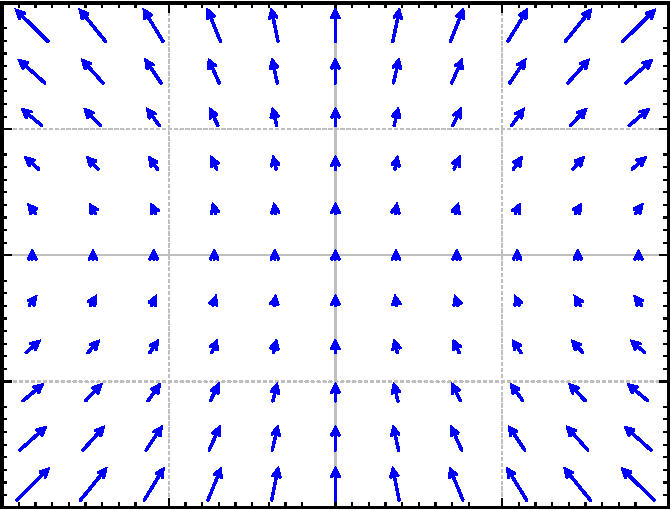
\includegraphics[width=1.75in]{figures/nlin-exer-xy-1py2}}
%mbxSTARTIGNORE
\task
%mbxENDIGNORE
%mbx \quad b) 
\parbox[c]{1.75in}{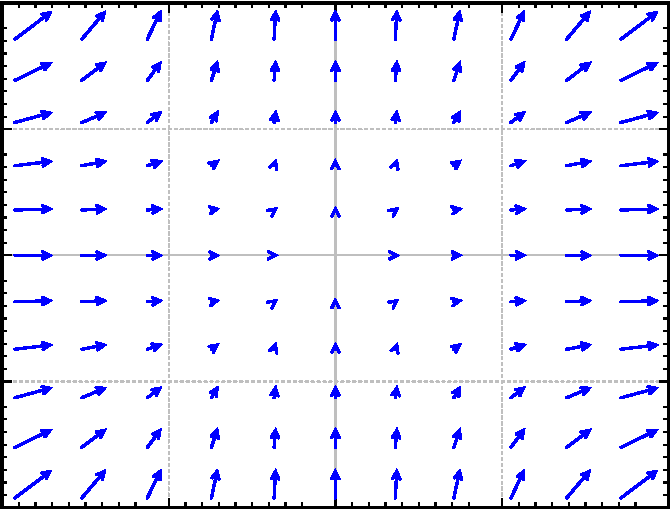
\includegraphics[width=1.75in]{figures/nlin-exer-x2-y2}}
%mbxSTARTIGNORE
\task
%mbxENDIGNORE
%mbx \quad c) 
\parbox[c]{1.75in}{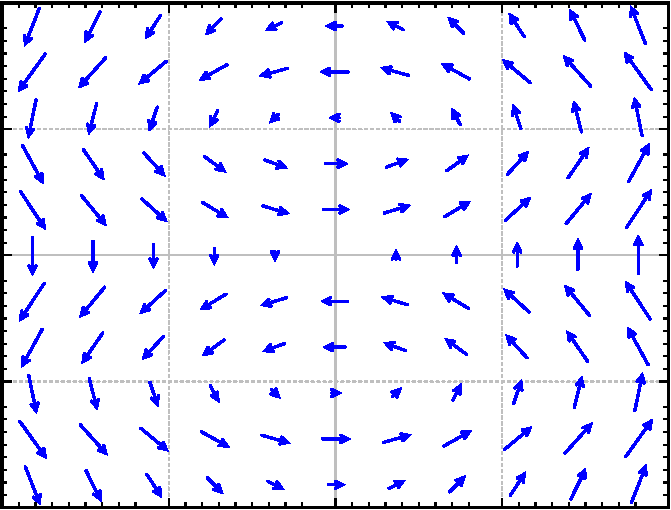
\includegraphics[width=1.75in]{figures/nlin-exer-sinpiy-x}}
%mbxSTARTIGNORE
\end{tasks}
%mbxENDIGNORE
\end{exercise}
\end{samepage}


\begin{exercise}
Find the critical points and linearizations of the following systems.
\begin{tasks}(2)
\task $x'=x^2-y^2$, \enspace $y'=x^2+y^2-1$,
\task $x'=-y$, \enspace $y'=3x+yx^2$,
\task $x'=x^2+y$, \enspace $y'=y^2+x$.
\end{tasks}
\end{exercise}

\begin{exercise}
For the following systems, verify they have critical point at $(0,0)$,
and find the linearization at $(0,0)$.
\begin{tasks}(2)
\task $x'=x+2y+x^2-y^2$, \enspace $y'=2y-x^2$
\task $x'=-y$, \enspace $y'=x-y^3$
\task* $x'=ax+by+f(x,y)$, $y'=cx+dy+g(x,y)$, where
$f(0,0) = 0$,
$g(0,0) = 0$, and all first partial derivatives of $f$ and $g$ are
also zero at $(0,0)$, that is,
$\frac{\partial f}{\partial x}(0,0) = 
\frac{\partial f}{\partial y}(0,0) = 
\frac{\partial g}{\partial x}(0,0) = 
\frac{\partial g}{\partial y}(0,0) = 0$.
\end{tasks}
\end{exercise}

\begin{exercise}
Take $x'=(x-y)^2$, \enspace $y'=(x+y)^2$. 
\begin{tasks}
\task Find the set of critical points.
\task Sketch a phase diagram and describe the behavior near the critical
point(s).
\task Find the linearization.  Is it helpful in understanding the system?
\end{tasks}
\end{exercise}

\begin{exercise}
Take $x'=x^2$, \enspace $y'=x^3$.
\begin{tasks}
\task Find the set of critical points.
\task Sketch a phase diagram and describe the behavior near the critical
point(s).
\task Find the linearization.  Is it helpful in understanding the system?
\end{tasks}
\end{exercise}

\setcounter{exercise}{100}

\pagebreak[2]
\begin{exercise}
Find the critical points and linearizations of the following systems.
\begin{tasks}(2)
\task $x'=\sin(\pi y)+(x-1)^2$, \enspace $y'=y^2-y$,
\task $x'=x+y+y^2$, \enspace $y'=x$,
\task $x'=(x-1)^2+y$, \enspace $y'=x^2+y$.
\end{tasks}
\end{exercise}
\exsol{%
a) Critical points $(0,0)$ and $(0,1)$.  At $(0,0)$ using $u=x$, $v=y$ the linearization is $u'=-2u-(\nicefrac{1}{\pi})v$, $v'=-v$.
At $(0,1)$ using $u=x$, $v=y-1$ the linearization is
$u'=-2u+(\nicefrac{1}{\pi})v$, $v'=v$.\\
b) Critical point $(0,0)$.  Using $u=x$, $v=y$ the linearization is
$u'=u+v$, $v'=u$.\\
c) Critical point $(\nicefrac{1}{2},\nicefrac{-1}{4})$.  Using
$u=x-\nicefrac{1}{2}$, $v=y+\nicefrac{1}{4}$ the linearization is
$u'=-u+v$, $v'=u+v$.
}

\begin{exercise}
Match systems
\begin{tasks}[counter-format=tsk[1])](2)
\task $x'=y^2$, \enspace $y'=-x^2$,
\task $x'=y$, \enspace $y'=(x-1)(x+1)$,
\task $x'=y+x^2$, \enspace $y'=-x$,
\end{tasks}
to the vector fields below.  Justify.
%mbxSTARTIGNORE
\begin{tasks}(3)
\task
%mbxENDIGNORE
%mbx \\
%mbx a)
\parbox[c]{1.75in}{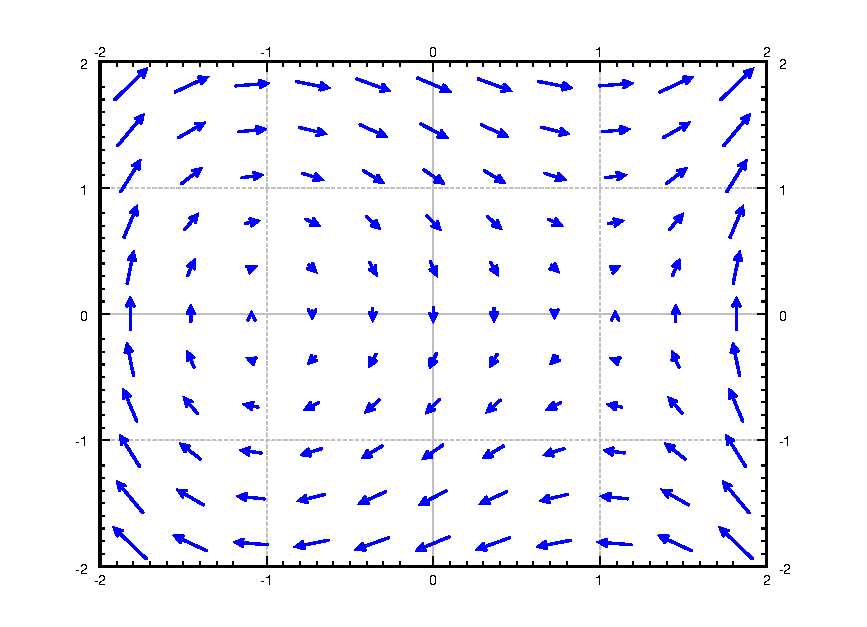
\includegraphics[width=1.75in]{figures/nlin-exer-y-xm1xp1}}
%mbxSTARTIGNORE
\task
%mbxENDIGNORE
%mbx \quad b)
\parbox[c]{1.75in}{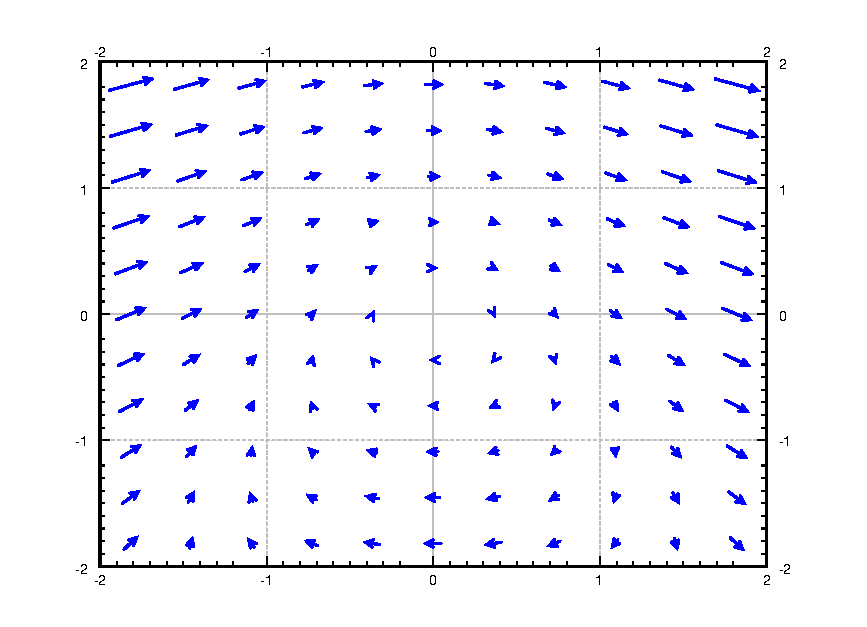
\includegraphics[width=1.75in]{figures/nlin-exer-ypx2-mx}}
%mbxSTARTIGNORE
\task
%mbxENDIGNORE
%mbx \quad c)
\parbox[c]{1.75in}{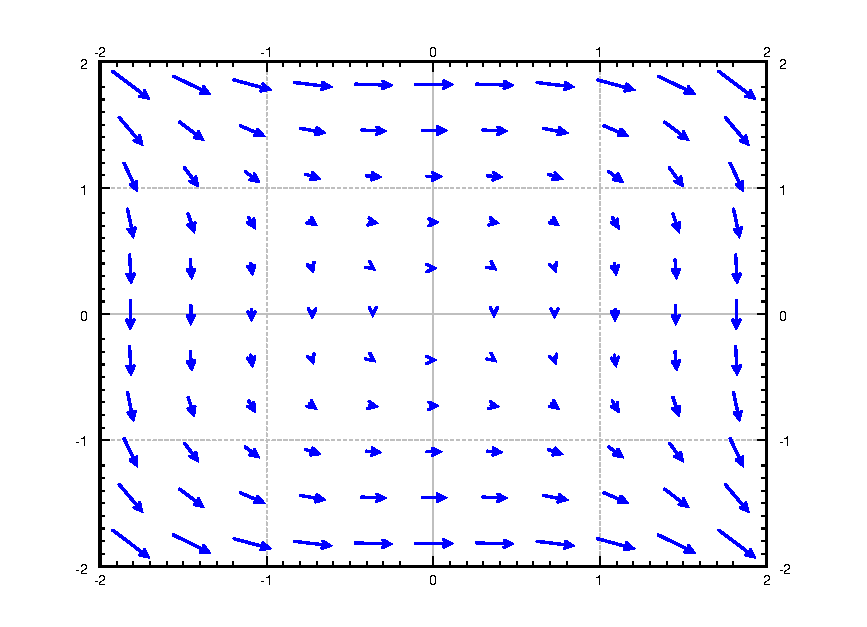
\includegraphics[width=1.75in]{figures/nlin-exer-y2-mx2}}
%mbxSTARTIGNORE
\end{tasks}
%mbxENDIGNORE
\end{exercise}
\exsol{%
1) is c), 2) is a), 3) is b)
}


\begin{samepage}
\begin{exercise}
The idea of critical points and linearization works in higher dimensions as
well.  You simply make the Jacobian matrix bigger by adding more functions
and more variables.  For the following system
of 3 equations find the critical points and their linearizations:
\begin{equation*}
x' = x + z^2, \qquad y' = z^2-y, \qquad z' = z+x^2.
\end{equation*}
\end{exercise}
\end{samepage}
\exsol{%
Critical points are $(0,0,0)$, and
$(-1, 1, -1)$.
The linearization at the origin using variables $u=x$, $v=y$, $w=z$ is
$u' = u$, $v'=-v$, $z' = w$.
The linearization at the point $(-1,1,-1)$ using variables $u=x+1$,
$v=y-1$, $w=z+1$ is
%$x=u-1$
%$y=v+1$
%$z=w-1$
%$u' = u-1 + (w-1)^2$, $v' = (w-1)^2-v+1$, $w' = (w-1)+(u-1)^2$.
%$u' = u + w^2-2w$, $v' = w^2-2w-v$, $w' = w+u^2-2u$
$u'=u-2w$, $v'=-v-2w$, $w'=w-2u$.
}

\begin{exercise}
Any two-dimensional non-autonomous system $x'=f(x,y,t)$, $y'=g(x,y,t)$ can
be written as a three-dimensional autonomous system (three equations).  Write down this
autonomous system using the variables $u$, $v$, $w$.
\end{exercise}
\exsol{%
$u' = f(u,v,w)$, $v'=g(u,v,w)$, $w' = 1$.
}

%%%%%%%%%%%%%%%%%%%%%%%%%%%%%%%%%%%%%%%%%%%%%%%%%%%%%%%%%%%%%%%%%%%%%%%%%%%%%%

\sectionnewpage
\section{Stability and classification of isolated critical points}
\label{nlinstability:section}

\sectionnotes{1.5--2 lectures\EPref{, \S6.1--\S6.2 in \cite{EP}}\BDref{,
\S9.2--\S9.3 in \cite{BD}}}

\subsection{Isolated critical points and almost linear systems}

A critical point is
\emph{isolated}\index{isolated critical point}
if it is the only critical point in some small
\myquote{neighborhood} of the point.  That is, if we zoom in far enough it is the
only critical point we see.  In the above example, the critical point was
isolated.  If on the other hand there would be a whole curve of critical
points, then it would not be isolated.

A system is called \emph{\myindex{almost linear}} at a critical point
$(x_0,y_0)$, if the critical point is isolated and the Jacobian matrix at the point
is invertible, or equivalently if the linearized system has an isolated
critical point.  In such a case, the nonlinear terms are very small
and the system behaves like its linearization, at least if we are close
to the critical point.

For example, the system in
Examples~\ref{example:nlin-1b-example} and \ref{example:nlin-1b-examplelin}
has two isolated critical points $(0,0)$ and $(0,1)$, and
is almost linear at both critical points as 
the Jacobian matrices at both points,
$\left[ \begin{smallmatrix} 0 & 1 \\ -1 & 0 \end{smallmatrix} \right]$ and
$\left[ \begin{smallmatrix} 0 & 1 \\ 1 & 0 \end{smallmatrix} \right]$,
are invertible.

On the other hand, the system $x' = x^2$, $y' = y^2$ has an isolated
critical point at $(0,0)$, however the Jacobian matrix
\begin{equation*}
\begin{bmatrix} 2x & 0 \\ 0 & 2y \end{bmatrix}
\end{equation*}
is zero when $(x,y) = (0,0)$.  So the system is not almost
linear.
Even a worse example is the system $x' = x$, $y' = x^2$, which does not have 
isolated critical points; $x'$ and $y'$ are both zero
whenever $x=0$, that is, the entire $y$-axis.

Fortunately, most often critical
points are isolated, and the system is almost linear at the critical
points.  So if we learn what happens there, we will have figured out the majority
of situations that arise in applications.



\subsection{Stability and classification of isolated critical points}

Once we have an isolated critical point, the system is almost linear at
that critical point, and we computed the
associated linearized system, we can classify what happens to the 
solutions.  We more or less use the classification for linear
two-variable systems from \sectionref{sec:twodimaut}, with one minor
caveat.
Let us list the behaviors depending on the eigenvalues of
the Jacobian matrix at the critical point in \tablevref{pln:behtab2}.
This table is very similar to \tablevref{pln:behtab}, with
the exception of missing \myquote{center} points.
%There is also a new column
%that we will discuss.
We will discuss centers later, as they are more complicated.

\begin{table}[h!t]
\mybeginframe
\capstart
\begin{center}
\begin{tabular}{@{}lll@{}}
\toprule
Eigenvalues of the Jacobian matrix & Behavior & Stability \\
\midrule
real and both positive & source / unstable node & unstable \\
real and both negative & sink / stable node & asymptotically stable \\
real and opposite signs & saddle & unstable \\
complex with positive real part & spiral source & unstable \\
complex with negative real part & spiral sink & asymptotically stable \\
\bottomrule
\end{tabular}
\end{center}
\caption{Behavior of an almost linear system near an isolated critical
point.  \label{pln:behtab2}}
\myendframe
\end{table}

In the third column,
we mark points as \emph{asymptotically stable} or \emph{unstable}.  Formally, a
\emph{\myindex{stable critical point}} $(x_0,y_0)$ is one where given any small distance $\epsilon$ to
$(x_0,y_0)$, and any initial condition within a perhaps smaller radius
around $(x_0,y_0)$, the trajectory
of the system never goes further away from $(x_0,y_0)$ than $\epsilon$.
An \emph{\myindex{unstable critical point}} is one that is not stable.
Informally, a point is stable if we start close to a critical point and
follow a trajectory we either go towards, or at least not away
from,
this critical point.

A stable critical point $(x_0,y_0)$ is called \emph{\myindex{asymptotically stable}} if
given any initial condition sufficiently close to $(x_0,y_0)$ and any
solution $\bigl( x(t), y(t) \bigr)$ satisfying that condition, then
\begin{equation*}
\lim_{t \to \infty} \bigl( x(t), y(t) \bigr) = (x_0,y_0) .
\end{equation*}
That is, the critical point is asymptotically stable
if any trajectory for a sufficiently close initial condition
goes towards the critical point $(x_0,y_0)$.

\begin{example} \label{example:nlin-xplusy}
Consider
$x'=-y-x^2$,
$y'=-x+y^2$.
See \figurevref{fig:nlin-ex813-new} for the phase diagram.
Let us find the critical points.  These are the points where
$-y-x^2 = 0$ and $-x+y^2=0$.  The first equation means $y = -x^2$, and
so $y^2 = x^4$.  Plugging into the second equation we obtain 
$-x+x^4 = 0$.  Factoring we obtain $x(1-x^3)=0$.  Since we are looking only
for real solutions we get either $x=0$ or $x=1$.  Solving for the
corresponding $y$ using $y = -x^2$, we get two critical points, one being $(0,0)$
and the other being $(1,-1)$.  Clearly the critical points are isolated.

\begin{myfig}
\capstart
\diffyincludegraphics{width=3in}{width=4.5in}{nlin-ex813-new}
\caption{The phase portrait with few sample trajectories of 
$x'=-y-x^2$, $y'=-x+y^2$.  \label{fig:nlin-ex813-new}}
\end{myfig}


Let us compute the Jacobian matrix:
\begin{equation*}
\begin{bmatrix}
-2x & -1 \\
-1 & 2y
\end{bmatrix} .
\end{equation*}
At the point $(0,0)$ we get the matrix
$\left[ \begin{smallmatrix} 0 & -1 \\ -1 & 0 \end{smallmatrix} \right]$ and
so the two eigenvalues are $1$ and $-1$.  As the matrix is invertible, the system is almost linear
at $(0,0)$.  As the eigenvalues are real
and of opposite signs, we get a saddle point, which is an unstable
equilibrium point.

At the point $(1,-1)$ we get the matrix
$\left[ \begin{smallmatrix} -2 & -1 \\ -1 & -2 \end{smallmatrix} \right]$ and
computing the eigenvalues we get $-1$, $-3$.
The matrix is invertible, and so the system is almost linear at $(1,-1)$.
As we have real eigenvalues and both negative, the critical
point is a sink, and therefore an asymptotically stable equilibrium point.
That is, if we start with any point $(x_i,y_i)$ close to $(1,-1)$ as
an initial condition and plot a trajectory, it approaches $(1,-1)$.
In other words,
\begin{equation*}
\lim_{t \to \infty} \bigl( x(t), y(t) \bigr) = (1,-1) .
\end{equation*}
As you can 
see from the diagram, this behavior is true even for some
initial points quite far from $(1,-1)$, but it is definitely not true for all
initial points.
\end{example}

\begin{example} \label{example:nlin-withexp}
Let us look at
$x'=y+y^2e^x$,
$y'=x$.  First let us find the critical points.  These are the points where
$y+y^2e^x = 0$ and $x=0$.  Simplifying we get $0=y+y^2 = y(y+1)$.  So the
critical points are $(0,0)$ and $(0,-1)$, and hence are isolated.  Let us
compute the Jacobian matrix:
\begin{equation*}
\begin{bmatrix}
y^2e^x & 1+2ye^x \\
1 & 0
\end{bmatrix}.
\end{equation*}

At the point $(0,0)$ we get the matrix
$\left[ \begin{smallmatrix} 0 & 1 \\ 1 & 0 \end{smallmatrix} \right]$ and
so the two eigenvalues are $1$ and $-1$.  As the matrix is invertible, the system is almost linear
at $(0,0)$.  And, as the eigenvalues are real
and of opposite signs, we get a saddle point, which is an unstable
equilibrium point.

At the point $(0,-1)$ we get the matrix
$\left[ \begin{smallmatrix} 1 & -1 \\ 1 & 0 \end{smallmatrix} \right]$ whose
eigenvalues are $\frac{1}{2} \pm i \frac{\sqrt{3}}{2}$.
The matrix is invertible, and so the system is almost linear at $(0,-1)$.
As we have complex eigenvalues with positive real part, the critical
point is a spiral source, and therefore an unstable equilibrium point.

\begin{myfig}
\capstart
\diffyincludegraphics{width=3in}{width=4.5in}{nlin-ex813}
\caption{The phase portrait with few sample trajectories of 
$x'=y+y^2e^x$, $y'=x$.  \label{fig:nlin-ex813}}
\end{myfig}

See \figurevref{fig:nlin-ex813} for the phase diagram.  Notice the two
critical points, and the behavior of the arrows in the vector field around
these points.
\end{example}

\subsection{The trouble with centers}

Recall, a linear system with a center means that trajectories
travel in closed elliptical orbits
in some direction around the critical point.  Such
a critical point we call a \emph{\myindex{center}} or
a \emph{\myindex{stable center}}.  It is not an asymptotically 
stable critical point, as the trajectories never approach the critical
point, but at least if you start sufficiently close to the critical point,
you stay close to the critical point.  The simplest example of such
behavior is the linear system with a center.  Another
example is the critical point $(0,0)$ in
\examplevref{example:nlin-1b-example}.

The trouble with a center in a nonlinear system is that whether the
trajectory goes towards or away from the critical point is governed by the
sign of the real part of the eigenvalues of the Jacobian matrix, and the Jacobian
matrix
in a nonlinear system changes from point to point.  Since this real
part is zero at the critical point itself, it can have either sign nearby,
meaning the trajectory could be pulled towards or away from the critical
point.

\begin{example}
An example of such a problematic behavior is the system
$x'=y, y' = -x+y^3$.  The only critical point
is the origin $(0,0)$.  The Jacobian matrix is 
\begin{equation*}
\begin{bmatrix}
0 & 1 \\
-1 & 3 y^2 \\
\end{bmatrix} .
\end{equation*}
At 
$(0,0)$ the Jacobian matrix is
$\left[ \begin{smallmatrix}
0 & 1 \\
-1 & 0 \\
\end{smallmatrix} \right]$, which has eigenvalues $\pm i$.  So the
linearization has a center.

Using the quadratic equation, the eigenvalues of the
Jacobian matrix at any point $(x,y)$ are
\begin{equation*}
\lambda = 
\frac{3}{2}y^2 \pm
i
\frac{\sqrt{4-9y^4}}{2} .
\end{equation*}
At any point where $y \not= 0$ (so at most points near the origin), the eigenvalues have a positive real part ($y^2$ can
never be negative).  This positive real part 
pulls the trajectory away from the origin.  A sample trajectory for an
initial condition near the origin is given in
\figurevref{fig:nlin-unstable-center}.
\begin{myfig}
\capstart
\diffyincludegraphics{width=3in}{width=4.5in}{nlin-unstable-centerfig}
\caption{An unstable critical point (spiral source) at the origin
for $x'=y, y' = -x+y^3$, even if the linearization has a center.  \label{fig:nlin-unstable-center}}
\end{myfig}
\end{example}

The moral of the example is that further analysis is needed when the
linearization has a center.  The analysis will in general be more
complicated than in the above example, and is more likely to involve
case-by-case consideration.  Such a complication should not be
surprising to you.  By now in your mathematical career, you have
seen many places where a simple test is inconclusive, recall for example
the second derivative test for maxima or minima, and requires more careful,
and perhaps ad hoc analysis of the situation.

\subsection{Conservative equations}

An equation of the form
\begin{equation*}
x'' + f(x) = 0
\end{equation*}
for an arbitrary function $f(x)$ is called a
\emph{\myindex{conservative equation}}.  For example the pendulum equation
is a conservative equation.  The equations are conservative as there is no
friction in the system so the energy in the system is \myquote{conserved.}
Let us write this equation as a
system of nonlinear ODE.
\begin{equation*}
x' = y, \qquad y' = -f(x) .
\end{equation*}
These types of equations have the
advantage that we can solve for their trajectories easily.

The trick is to first think of $y$ as a function of $x$ for a moment.  Then
use the chain rule
\begin{equation*}
x'' = y' = \frac{dy}{dx} x' = y \frac{dy}{dx} ,
\end{equation*}
where the prime indicates a derivative with respect to $t$.  
We obtain $y \frac{dy}{dx} + f(x) = 0$.  We integrate with respect to
$x$ to get
$\int y \frac{dy}{dx} \,dx + \int f(x)\, dx = C$.  In other words
\begin{equation*}
\frac{1}{2} y^2  + \int f(x)\, dx = C .
\end{equation*}
We obtained an implicit equation for the trajectories, with different $C$
giving different trajectories.  The value of
$C$ is conserved on any trajectory.  This expression is
sometimes called the \emph{\myindex{Hamiltonian}} or the energy of the
system.
If you look back to \sectionref{exact:section}, you will notice
that $y\frac{dy}{dx} + f(x) = 0$ is an exact equation, and
we just found a potential function.

\begin{example}
Let us find the trajectories for the equation $x'' + x-x^2 = 0$,
which is the equation from
\examplevref{example:nlin-1b-example}.  The corresponding
first order system is
\begin{equation*}
x' = y , \qquad y' = -x+x^2 .
\end{equation*}
Trajectories satisfy
\begin{equation*}
\frac{1}{2} y^2  + \frac{1}{2} x^2 - \frac{1}{3} x^3  = C .
\end{equation*}
We solve for $y$
\begin{equation*}
y = \pm \sqrt{-x^2 + \frac{2}{3} x^3  + 2C} .
\end{equation*}

Plotting these graphs we get exactly the trajectories in 
\figurevref{fig:nlin-1b}.  In particular we notice that near the origin
the trajectories are \emph{\myindex{closed curves}}: they keep going
around the origin, never spiraling in or out.  Therefore we discovered a way
to verify that the critical point at $(0,0)$ is a stable center.
The critical point at $(0,1)$ is a saddle as we already noticed.
This example is typical for conservative equations.
\end{example}

Consider an arbitrary
conservative equation $x'' + f(x) = 0$.
All critical points occur when $y=0$ (the
$x$-axis), that is when $x' = 0$.  The critical points are 
those points on the $x$-axis where $f(x) = 0$.
The trajectories are given by
\begin{equation*}
y = \pm \sqrt{ - 2 \int f(x)\, dx + 2C} .
\end{equation*}
So all trajectories are mirrored across the $x$-axis.  In particular,
there can be no spiral sources nor sinks.
The Jacobian matrix is
\begin{equation*}
\begin{bmatrix}
0 & 1 \\
-f'(x) & 0
\end{bmatrix} .
\end{equation*}
The critical point is almost linear if $f'(x) \not= 0$ at the critical 
point.  Let $J$ denote the Jacobian matrix.
The eigenvalues of $J$ are solutions to
\begin{equation*}
0 = \det(J - \lambda I) = \lambda^2 + f'(x) .
\end{equation*}
Therefore $\lambda = \pm \sqrt{-f'(x)}$.  In other words, either we get
real eigenvalues of opposite signs (if $f'(x) < 0$),
or we get purely imaginary eigenvalues (if $f'(x) > 0$).
There are only two possibilities for critical points, either an \emph{unstable
saddle point}, or a \emph{stable center}.
There are never any sinks or sources.

\subsection{Exercises}

\begin{exercise}
For the systems below, find and classify the critical points, also indicate
if the equilibria are stable, asymptotically stable, or unstable.
\begin{tasks}(2)
\task $x'=-x+3x^2, y'=-y$
\task $x'=x^2+y^2-1$, $y'=x$
\task $x'=ye^x$, $y'=y-x+y^2$
\end{tasks}
\end{exercise}

\begin{exercise}
Find the implicit equations of the trajectories of the following
conservative systems.  Next find their critical points (if any) and classify them.
\begin{tasks}(2)
\task $x''+ x+x^3 = 0$
\task $\theta''+\sin \theta = 0$
\task $z''+ (z-1)(z+1) = 0$
\task $x''+ x^2+1 = 0$
\end{tasks}
\end{exercise}

\begin{exercise}
Find and classify the critical point(s) of $x' = -x^2$, $y' = -y^2$.
\end{exercise}

\begin{samepage}
\begin{exercise}
Suppose $x'=-xy$, $y'=x^2-1-y$.
\begin{tasks}
\task
Show there are two spiral sinks at
$(-1,0)$ and $(1,0)$.
\task
For any initial point of the form $(0,y_0)$, find what is the trajectory.
\task
Can a trajectory starting at $(x_0,y_0)$ where $x_0 > 0$ spiral into 
the critical point at $(-1,0)$?  Why or why not?
\end{tasks}
\end{exercise}
\end{samepage}

\begin{exercise} \label{exercise:increasing}
In the example $x'=y$, $y'=y^3-x$ show that for any trajectory, the distance
from the origin is an increasing function.
Conclude
that the origin behaves like is a spiral source.
Hint: Consider $f(t) =
{\bigl(x(t)\bigr)}^2 + 
{\bigl(y(t)\bigr)}^2$ and show it has positive derivative.
\end{exercise}


\begin{exercise}
Suppose $f$ is always positive.
Find the trajectories of $x''+f(x') = 0$.
Are there any critical points?
\end{exercise}

\begin{exercise}
Suppose that $x' = f(x,y)$, $y' = g(x,y)$.  Suppose that $g(x,y) > 1$ for
all $x$ and $y$.  Are there any critical points?  What can we say about the
trajectories at $t$ goes to infinity?
\end{exercise}

\setcounter{exercise}{100}

\begin{exercise}
For the systems below, find and classify the critical points.
\begin{tasks}(3)
\task $x'=-x+x^2$, $y'=y$
\task $x'=y-y^2-x$, $y'=-x$
\task $x'=xy$, $y'=x+y-1$
\end{tasks}
\end{exercise}
\exsol{%
a) $(0,0)$: saddle (unstable), $(1,0)$: source (unstable), \qquad
b) $(0,0)$: spiral sink (asymptotically stable), $(0,1)$: saddle (unstable), \qquad
c) $(1,0)$: saddle (unstable), $(0,1)$: saddle (unstable)
}

\begin{exercise}
Find the implicit equations of the trajectories of the following
conservative systems.  Next find their critical points (if any) and classify them.
\begin{tasks}(3)
\task $x''+ x^2 = 4$
\task $x''+ e^x = 0$
\task $x''+ (x+1)e^x = 0$
\end{tasks}
\end{exercise}
\exsol{%
a) $\frac{1}{2}y^2 + \frac{1}{3}x^3 -4x = C$, critical points
$(-2,0)$: an unstable saddle, and $(2,0)$: a stable center.
b) $\frac{1}{2}y^2 + e^x = C$, no critical points.
c) $\frac{1}{2}y^2 + xe^x = C$, critical point at $(-1,0)$ is a stable center.
}

\begin{exercise}
The conservative system $x''+x^3 = 0$ is not almost linear.  Classify
its critical point(s) nonetheless.
\end{exercise}
\exsol{%
Critical point at $(0,0)$.
Trajectories are $y = \pm \sqrt{2C+(\nicefrac{1}{2})x^4}$, for $C > 0$, these give closed
curves around the origin, so the critical point is a stable center.
}

\begin{exercise}
Derive an analogous classification of critical points for equations in one dimension,
such as $x'= f(x)$ based on the derivative.  A point $x_0$ is critical when $f(x_0) = 0$ and
almost linear if in addition $f'(x_0) \not= 0$.  Figure out if the critical point is stable or unstable
depending on the sign of $f'(x_0)$.  Explain.  Hint: see \sectionref{auteq:section}.
\end{exercise}
\exsol{%
A critical point $x_0$ is stable if $f'(x_0) < 0$ and unstable when $f'(x_0)
> 0$.
}

%%%%%%%%%%%%%%%%%%%%%%%%%%%%%%%%%%%%%%%%%%%%%%%%%%%%%%%%%%%%%%%%%%%%%%%%%%%%%%

\sectionnewpage
\section{Applications of nonlinear systems}
\label{nlinapps:section}

\sectionnotes{2 lectures\EPref{, \S6.3--\S6.4 in \cite{EP}}\BDref{, \S9.3,
\S9.5 in \cite{BD}}}

In this section we study two very standard examples of nonlinear
systems.  First, we look at the nonlinear pendulum equation.  We saw
the pendulum equation's linearization before, but we noted it
was only valid for small angles and short times.  Now we find out what
happens for large angles.  Next, we look at the predator-prey equation,
which finds various applications in modeling problems in biology, chemistry,
economics, and elsewhere.

\subsection{Pendulum}

The first example we study is the pendulum equation
$\theta''+\frac{g}{L} \sin \theta = 0$.  Here, $\theta$ is the angular
displacement, $g$ is the gravitational constant, and $L$ is the length of
the pendulum.  In this equation we disregard friction, so we are talking
about an idealized pendulum.

%8 is the number of lines, should be adjusted
\begin{mywrapfigsimp}[8]{1.45in}{1.75in}
\noindent
\inputpdft{mv-pend}
\end{mywrapfigsimp}
This equation is a conservative
equation, so we can use our analysis of conservative equations
from the previous section.
Let us change the equation to a two-dimensional
system in variables $(\theta,\omega)$ by introducing the new
variable $\omega$:
\begin{equation*}
\begin{bmatrix}
\theta \\ \omega
\end{bmatrix} '
=
\begin{bmatrix}
\omega \\
- \frac{g}{L} \sin \theta
\end{bmatrix} .
\end{equation*}
The critical points of this system are when $\omega = 0$ and $-\frac{g}{L}
\sin \theta = 0$, or in other words if $\sin \theta = 0$.  So the critical
points are when $\omega = 0$ and $\theta$ is a multiple of $\pi$.  That is,
the points are $\ldots (-2\pi,0), (-\pi,0), (0,0), (\pi,0), (2\pi,0)
\ldots$.  While there are infinitely many critical points, they are all isolated.
Let us compute the Jacobian matrix:
\begin{equation*}
\begin{bmatrix}
\frac{\partial}{\partial \theta} \Bigl( \omega \Bigr) & 
\frac{\partial}{\partial \omega} \Bigl( \omega \Bigr) \\
\frac{\partial}{\partial \theta} \Bigl( - \frac{g}{L} \sin \theta \Bigr) & 
\frac{\partial}{\partial \omega} \Bigl( - \frac{g}{L} \sin \theta \Bigr)
\end{bmatrix}
=
\begin{bmatrix}
0 & 1 \\
- \frac{g}{L} \cos \theta & 0
\end{bmatrix} .
\end{equation*}

For conservative equations, there are two types of
critical points.  Either stable centers, or saddle points.  The eigenvalues
of the Jacobian matrix are $\lambda = \pm \sqrt{-\frac{g}{L}\cos \theta}$.

The
eigenvalues are going to be real when $\cos \theta < 0$.  This happens at the odd multiples of $\pi$.
The
eigenvalues are going to be purely imaginary 
when $\cos \theta > 0$.  This happens at the even
multiples of $\pi$.  Therefore the system has a stable center at
the points $\ldots (-2\pi,0), (0,0), (2\pi,0) \ldots$, and it has an
unstable saddle at
the points $\ldots (-3\pi,0), (-\pi,0), (\pi,0), (3\pi,0) \ldots$.  Look at the
phase diagram in \figurevref{fig:nlin-pend-phasediag},
where for simplicity we let $\frac{g}{L} = 1$.

\begin{myfig}
\capstart
\diffyincludegraphics{width=3in}{width=4.5in}{nlin-pend-phasediag}
\caption{Phase plane diagram and some trajectories of
the nonlinear pendulum equation. \label{fig:nlin-pend-phasediag}}
\end{myfig}

In the linearized equation we have only a single critical point, the center
at $(0,0)$.  Now we see more clearly what we meant when we said the
linearization is good for small angles.  The horizontal axis is the
deflection angle.  The vertical axis is the angular velocity of the
pendulum.  Suppose we start at $\theta = 0$ (no deflection), and
we start with a small angular velocity $\omega$.  Then the trajectory keeps going
around the critical point $(0,0)$ in an approximate circle.  This
corresponds to short swings of the pendulum back and forth.  When $\theta$
stays small, the trajectories really look like circles and hence are very
close to our linearization.

When we give the pendulum a big enough push, it
goes across the top and keeps spinning about its axis.  This behavior
corresponds to the
wavy curves that do not cross the horizontal axis in the phase diagram.
Let us suppose we look at the top curves, when the angular velocity $\omega$
is large and positive.  Then the pendulum is going
around and around its axis.  The velocity is going to
be large when the pendulum is near the bottom, and the velocity is the
smallest when the pendulum
is close to the top of its loop.

At each critical point, there is an equilibrium solution.  Consider
the solution
$\theta = 0$;  the pendulum is not moving
and is hanging straight down.  This is a stable place for the
pendulum to be, hence this is a \emph{stable} equilibrium.

The other type of equilibrium solution is at the unstable point, for example
$\theta = \pi$.  Here the pendulum is upside down.  Sure you can balance the
pendulum this way and it will stay, but this is an \emph{unstable} equilibrium.
Even the tiniest push will make the pendulum start swinging wildly.

See \figurevref{fig:nlin-pend} for a diagram.  The first picture is the
stable equilibrium $\theta = 0$.  The second picture corresponds to those
\myquote{almost circles} in the phase diagram around $\theta =0$ when the angular
velocity is small.  The next picture is the unstable equilibrium $\theta =
\pi$.  The last picture corresponds to the wavy lines for large angular
velocities.

\begin{myfig}
\capstart
\inputpdft{nlin-pend}
\caption{Various possibilities for the motion of the pendulum. \label{fig:nlin-pend}}
\end{myfig}

The quantity 
\begin{equation*}
\frac{1}{2} \omega^2  - \frac{g}{L} \cos \theta 
\end{equation*}
is conserved by any solution.  This is the energy or the Hamiltonian of
the system.

We have a conservative equation and so (exercise) the
trajectories are given by
\begin{equation*}
\omega = \pm \sqrt{ \frac{2g}{L} \cos \theta + C} ,
\end{equation*}
for various values of $C$.  
Let us look at the initial condition of $(\theta_0,0)$,
that is, we take the pendulum to
angle $\theta_0$, and just let it go (initial angular velocity 0).
We plug the initial conditions into the above and solve for $C$ to obtain
\begin{equation*}
C = - \frac{2g}{L} \cos \theta_0 .
\end{equation*}
Thus the expression for the trajectory is
\begin{equation*}
\omega = \pm \sqrt{ \frac{2g}{L}} \sqrt{ \cos \theta - \cos \theta_0 } .
\end{equation*}

Let us figure out the period.  That is, the time it takes for the pendulum
to swing back and forth.
We notice that the trajectory about the
origin in the phase plane is symmetric about both the $\theta$ and the
$\omega$-axis.  That is, in terms of $\theta$,
the time it takes from $\theta_0$ to $-\theta_0$
is the same as it takes from $-\theta_0$ back to $\theta_0$.  Furthermore,
the time it takes from $-\theta_0$ to $0$ is the same as to go from $0$ to
$\theta_0$.  Therefore, let us find how long it takes for
the pendulum to go from angle 0 to angle $\theta_0$, which is a quarter of
the full oscillation and then multiply by 4.

We figure out this time by finding
$\frac{dt}{d\theta}$ and integrating from $0$ to $\theta_0$.
The period is four times
this integral.  Let us stay in the region where $\omega$ is positive.
Since $\omega = \frac{d\theta}{dt}$, inverting we get
\begin{equation*}
\frac{dt}{d\theta} = \sqrt{\frac{L}{2g}} \frac{1}{\sqrt{\cos \theta - \cos \theta_0 }} .
\end{equation*}
Therefore the period $T$ is given by
\begin{equation*}
T = 4 \sqrt{\frac{L}{2g}} \int_0^{\theta_0} \frac{1}{\sqrt{\cos \theta -
\cos \theta_0 }}\, d\theta .
\end{equation*}
The integral is an improper integral, and we cannot in
general evaluate it symbolically.  We must resort to numerical
approximation if we want to compute a particular $T$.

Recall from \sectionref{sec:mv}, the linearized equation $\theta''+\frac{g}{L}\theta
= 0$ has period
\begin{equation*}
T_{\text{linear}} = 2\pi \sqrt{\frac{L}{g}} .
\end{equation*}
We plot $T$, $T_{\text{linear}}$, and the relative error
$\frac{T-T_{\text{linear}}}{T}$ in \figurevref{fig:TvsT0}.  The relative error
says how far is our approximation from the real period percentage-wise.
Note that $T_{\text{linear}}$ is simply a constant, it does not change with
the initial angle $\theta_0$.  The actual period $T$ gets larger and larger as
$\theta_0$ gets larger.
Notice how the relative error is small when $\theta_0$ is small.  It is
still only $15\%$ when $\theta_0 = \frac{\pi}{2}$, that is, a 90 degree
angle.  The error is $3.8\%$ when starting at $\frac{\pi}{4}$, 
a 45 degree angle.  At a 5 degree initial angle, the error is only $0.048 \%$.

\begin{myfig}
\capstart
%original files nlin-T-vs-T0-abs nlin-T-vs-T0-relerr
\diffyincludegraphics{width=6.24in}{width=9in}{nlin-T-vs-T0-abs-relerr}
\caption{The plot of $T$ and $T_{\text{linear}}$ with $\frac{g}{L} =
1$ (left), and the plot of the relative
error $\frac{T-T_{\text{linear}}}{T}$ (right), for $\theta_0$ between 0 and $\pi/2$. \label{fig:TvsT0}}
\end{myfig}

While it is not immediately obvious from the formula, it is true that
\begin{equation*}
\lim_{\theta_0 \uparrow \pi} T = \infty .
\end{equation*}
That is, the period goes to infinity as the initial angle approaches the
unstable equilibrium point.  So if we put the pendulum almost upside down it
may take a very long time before it gets down.  This is consistent with the
limiting behavior, where the exactly upside down pendulum never makes an
oscillation, so we could think of that as infinite period.

\subsection{Predator-prey or Lotka--Volterra systems}

One of the most common simple applications of nonlinear systems are the
so-called \emph{\myindex{predator-prey}} or
\emph{\myindex{Lotka--Volterra}}%
\footnote{Named for the American mathematician, chemist, and statistician
\href{https://en.wikipedia.org/wiki/Alfred_J._Lotka}{Alfred James Lotka}
(1880--1949) and the Italian mathematician and physicist
\href{https://en.wikipedia.org/wiki/Vito_Volterra}{Vito Volterra}
(1860--1940).}
systems.  For example, these systems arise 
when two species interact, one as the prey and one as the predator.  It is
then no surprise that the equations also see applications in economics.
The system also arises in chemical reactions.
In biology, this system of equations explains the natural periodic variations of populations of
different species in nature.  Before the application of differential
equations, these periodic variations in the population baffled biologists.

We keep
with the classical example of hares and foxes in a forest, it is the
easiest to understand.
\begin{equation*}
\begin{aligned}
& x = \# \text{ of hares (the prey),} \\
& y = \# \text{ of foxes (the predator).}
\end{aligned}
\end{equation*}
When there are a lot of hares, there is plenty of food for the foxes, so
the fox population grows.  However, when the fox population grows, the foxes
eat more hares, so when there are lots of foxes, the hare population
should go down, and vice versa.
The Lotka--Volterra model proposes that this 
behavior is described by the system of equations
\begin{equation*}
\begin{aligned}
& x' = (a-by)x, \\
& y' = (cx-d)y,
\end{aligned}
\end{equation*}
where $a,b,c,d$ are some parameters that describe the interaction of the
foxes and hares\footnote{This interaction does not end well for the
hare.}.  In this model, these are all positive numbers.

Let us analyze the idea behind this model.  The model is a slightly more
complicated idea based on the exponential population model.
First expand,
\begin{equation*}
x' = (a-by)x = ax - byx .
\end{equation*}
The hares are expected to simply grow exponentially in the absence of foxes,
that is where the $ax$ term comes in, the growth in population is
proportional to the population itself.  We are assuming the hares
always find enough food and have enough space to reproduce.  However,
there is another component $-byx$, that is, the population also is
decreasing proportionally to the number of foxes.  Together we can write the
equation as $(a-by)x$, so it is like exponential growth or decay but the
constant depends on the number of foxes.

The equation for foxes is very similar, expand again
\begin{equation*}
y' = (cx-d)y = cxy-dy .
\end{equation*}
The foxes need food (hares) to reproduce: the more food, the bigger the
rate of growth, hence the $cxy$ term.  On the other hand, there are 
natural deaths in the fox population, and hence the $-dy$ term.

Without further delay, let us start with an explicit example.  Suppose the
equations are 
\begin{equation*}
x' = (0.4-0.01y)x, \qquad y' = (0.003x-0.3)y .
\end{equation*}
See \figurevref{fig:nlin-pred-prey} for the phase portrait.  In this example
it makes sense to also plot $x$ and $y$ as graphs with respect to time.
Therefore the second graph in 
\figureref{fig:nlin-pred-prey} is the graph of $x$ and $y$ on the vertical
axis (the prey $x$ is the thinner line with taller peaks), against time
on the horizontal axis.  The particular solution graphed was with initial
conditions of 20 foxes and 50 hares.
\begin{myfig}
\capstart
%original files nlin-pred-prey-phase nlin-pred-prey-graphs
\diffyincludegraphics{width=6.24in}{width=9in}{nlin-pred-prey-phase-graphs}
\caption{The phase portrait (left) and graphs of $x$ and $y$ for
a sample solution (right). \label{fig:nlin-pred-prey}}
\end{myfig}

Let us analyze what we see on the graphs.  We work in the general
setting rather than putting in specific numbers.  We start with finding
the critical points.  Set $(a-by)x = 0$, and $(cx-d)y = 0$.
The first equation is satisfied if either $x=0$ or $y=\nicefrac{a}{b}$.  If $x=0$, the
second equation implies $y=0$.  If $y= \nicefrac{a}{b}$, the second equation implies
$x=\nicefrac{d}{c}$.
There are two equilibria: at $(0,0)$ when there are no animals at all, and at
$(\nicefrac{d}{c},\nicefrac{a}{b})$.  
In our specific example $x = \nicefrac{d}{c} = 100$, and $y = \nicefrac{a}{b} = 40$.
This is the point where there are 100 hares and 40 foxes.

We compute the Jacobian matrix:
\begin{equation*}
\begin{bmatrix}
a-by & -bx \\
cy & cx-d
\end{bmatrix} .
\end{equation*}
At the origin $(0,0)$ we get the matrix
$\left[ \begin{smallmatrix}
a & 0 \\
0 & -d
\end{smallmatrix} \right]$, so the eigenvalues are $a$ and $-d$, hence real
and of opposite signs.  So the critical point at the origin is a saddle.
This makes sense.  If you started with some foxes but no hares, then the
foxes would go extinct, that is, you would approach the origin.  If you
started with no foxes and a few hares, then the hares would keep multiplying
without check, and so you would go away from the origin.

OK, how about the other critical point at $(\nicefrac{d}{c},\nicefrac{a}{b})$.  Here
the Jacobian matrix becomes
\begin{equation*}
\begin{bmatrix}
0 & -\frac{bd}{c} \\
\frac{ac}{b} & 0
\end{bmatrix} .
\end{equation*}
The eigenvalues satisfy $\lambda^2 + ad = 0$.  In
other words, $\lambda = \pm i \sqrt{ad}$.  The eigenvalues being
purely imaginary, we are in the case where we cannot quite decide using only
linearization.  We could
have a stable center, spiral sink, or a spiral source.  That is, the
equilibrium could be asymptotically stable, stable, or unstable.  Of
course I gave you a picture above that seems to imply it is a stable
center.  But never trust a picture only.  Perhaps the oscillations
are getting larger and larger, but only \emph{very} slowly.  Of course this would be
bad as it would imply something will go wrong with our population
sooner or later.  And I only graphed a very specific example with very
specific trajectories.

How can we be sure we are in the stable situation?
As we said before, in the case of purely imaginary eigenvalues, we have to
do a bit more work.  Previously we found that for conservative systems,
there was a certain quantity that was conserved on the trajectories, and
hence the trajectories had to go in closed loops.
We can use a similar technique here.  We just have to figure out what is the
conserved quantity.  After some trial and error we find the
constant
\begin{equation*}
C = \frac{y^a x^d}{e^{cx+by}} = y^a x^d e^{-cx-by}
\end{equation*}
is conserved.  Such a quantity is called the \emph{\myindex{constant of
motion}}.  Let us check $C$ really is a constant of motion.  How do we check, you say?  Well, a constant is
something that does not change with time, so let us compute the derivative
with respect to time:
\begin{equation*}
C' = 
a y^{a-1}y' x^d e^{-cx-by}
+
y^a d x^{d-1} x' e^{-cx-by}
+
y^a x^d e^{-cx-by} (-cx'-by') .
\end{equation*}
Our equations give us what $x'$ and $y'$ are so let us plug those in:
\begin{equation*}
\begin{split}
C' & = 
a y^{a-1} (cx-d)y x^d e^{-cx-by}
+
y^a d x^{d-1} (a-by)x e^{-cx-by}
\\
& \phantom{mm} +
y^a x^d e^{-cx-by} \bigl(-c(a-by)x-b(cx-d)y\bigr)
\\
& =
y^a x^d e^{-cx-by}
\Bigl(
a (cx-d)
+
d (a-by)
+
\bigl(-c(a-by)x-b(cx-d)y\bigr) \Bigr)
\\
& = 
0 .
\end{split}
\end{equation*}
So along the trajectories $C$ is constant.  In fact, the expression $C =
\frac{y^a x^d}{e^{cx+by}}$ gives us an implicit equation for the
trajectories.  In any case, once we have found this constant of motion,
it must be true that the
trajectories are simple curves, that is, the level curves of
$\frac{y^a x^d}{e^{cx+by}}$.  It turns out, the critical point at
$(\nicefrac{d}{c},\nicefrac{a}{b})$ is a maximum for $C$ (left as an exercise).
So $(\nicefrac{d}{c},\nicefrac{a}{b})$ is a stable equilibrium point, and 
we do not have to worry about the foxes and hares going extinct or their
populations exploding.

One blemish on this wonderful model is that the number of foxes and hares
are discrete quantities and we are modeling with continuous variables.  Our
model has no problem with there being 0.1 fox in the forest for example,
while in reality that makes no sense.  The approximation is a reasonable one
as long as the number of foxes and hares are large, but it does not make
much sense for small numbers.  One must be careful in interpreting any
results from such a model.

An interesting consequence (perhaps counterintuitive) of this model is that adding animals to
the forest might lead to extinction, because the variations will get too
big, and one of the populations will get close to zero.  For example, suppose there are 20 foxes and 50 hares as
before, but now we bring in more foxes, bringing their number to 200.  If we
run the computation, we find the number of hares will plummet to just
slightly more than 1 hare in the whole forest.  In reality that most
likely means the hares die out, and then the foxes will die out as well
as they will have nothing to eat.

Showing that a system of equations has a stable solution can be a very
difficult problem.  When Isaac Newton put forth his laws of
planetary motions, he proved that a single planet orbiting a single sun is a
stable system.  But any solar system with more than 1 planet proved very
difficult indeed.  In fact, such a system behaves chaotically (see 
\sectionref{sec:chaos}), meaning small changes in initial conditions lead to very
different long-term outcomes.  From numerical experimentation and
measurements, we know the earth will not fly out into the empty space
or crash into the sun, for at least some millions of years or so.
But we do not know what happens beyond that.

\subsection{Exercises}

\begin{exercise}
Take the \emph{\myindex{damped nonlinear pendulum equation}} $\theta '' + \mu \theta' +
(\nicefrac{g}{L})
\sin \theta = 0$ for some $\mu > 0$ (that is, there is some friction).
\begin{tasks}
\task
Suppose $\mu = 1$ and $\nicefrac{g}{L} = 1$ for simplicity, find and
classify the critical points.
\task
Do the same for any $\mu > 0$ and any $g$
and $L$, but such that the damping is small, in particular, $\mu^2 <
4(\nicefrac{g}{L})$.
\task
Explain what your findings mean, and if it agrees with what you
expect in reality.
\end{tasks}
\end{exercise}

\begin{exercise}
Suppose the hares do not grow exponentially, but logistically.  In
particular consider
\begin{equation*}
x' = (0.4-0.01y)x - \gamma x^2, \qquad y' = (0.003x-0.3)y .
\end{equation*}
For the following two values of $\gamma$,
find and classify all the critical points in the positive quadrant, that is, for
$x \geq 0$ and $y \geq 0$.  Then sketch the phase diagram.  Discuss the
implication for the long term behavior of the population.
\begin{tasks}(2)
\task
$\gamma=0.001$, 
\task
$\gamma=0.01$.
\end{tasks}
\end{exercise}

\begin{exercise}
{\ }
\begin{tasks}
\task Suppose $x$ and $y$ are
positive variables.  Show $\frac{y x}{e^{x+y}}$
attains a maximum at $(1,1)$.
\task Suppose $a,b,c,d$ are positive constants, and also suppose $x$ and $y$ are
positive variables.  Show $\frac{y^a x^d}{e^{cx+by}}$
attains a maximum at $(\nicefrac{d}{c},\nicefrac{a}{b})$.
\end{tasks}
\end{exercise}

\begin{exercise}
Suppose that for the pendulum equation we take a trajectory giving the
spinning-around motion, for example $\omega = \sqrt{\frac{2g}{L} \cos \theta
+ \frac{2g}{L} + \omega_0^2}$.  This is the trajectory where the lowest
angular velocity is $\omega_0^2$.  Find an integral expression for how long it takes
the pendulum to go all the way around.
\end{exercise}

%Suppose we have the system predator-prey system where the foxes are also
%hunted at a constant rate $hy$ proportional to the population.  That is,
%$x' = (a-by)x,$  $y' = (cx-d)y - hy$.  Find and analyze the critical points.

\begin{exercise}[challenging]
Take the pendulum, suppose the initial position is $\theta = 0$.
\begin{tasks}
\task
Find the expression for $\omega$ giving the trajectory
with initial condition $(0,\omega_0)$.  Hint: Figure out what $C$
should be in terms of $\omega_0$.
\task
Find the crucial angular velocity $\omega_1$, such that
for any higher initial angular velocity,
the pendulum will keep going around its
axis, and for any lower initial angular velocity, the pendulum will simply
swing back and forth.
Hint: When the pendulum doesn't go over the top the expression for $\omega$
will be undefined for some $\theta$s.
\task
What do you think happens if the initial condition is $(0,\omega_1)$,
that is, the initial angle is 0, and the initial angular velocity is exactly
$\omega_1$.
\end{tasks}
\end{exercise}

\setcounter{exercise}{100}

\begin{exercise}
Take the damped nonlinear pendulum equation $\theta '' + \mu \theta' +
(\nicefrac{g}{L})
\sin \theta = 0$ for some $\mu > 0$ (that is, there is friction).
Suppose the friction is large, in particular $\mu^2 > 4 (\nicefrac{g}{L})$.
\begin{tasks}
\task
Find and classify the critical points.
\task
Explain what your findings mean, and if it agrees with what you
expect in reality.
\end{tasks}
\end{exercise}
\exsol{%
a) Critical points are $\omega=0$, $\theta=k\pi$ for any integer $k$.  When
$k$ is odd, we have a saddle point.  When $k$ is even we get a sink.  b)
The findings mean the pendulum will simply go to one of the sinks, for
example $(0,0)$ and it will not swing back and forth.  The friction is too high for it to
oscillate, just like an overdamped mass-spring system.
}

\begin{exercise}
Suppose we have the system predator-prey system where the foxes are also
killed at a constant rate $h$ ($h$ foxes killed per unit time):
$x' = (a-by)x,$  $y' = (cx-d)y - h$.
\begin{tasks}
\task Find the critical points and the
Jacobian matrices of the system.
\task Put in the constants $a=0.4$, $b=0.01$, $c=0.003$, $d=0.3$, $h=10$.
Analyze the critical points.  What do you think it says about the forest?
\end{tasks}
\end{exercise}
\exsol{%
a) Solving for the critical points we get
$(0,-\nicefrac{h}{d})$ and $(\frac{bh+ad}{ac},\frac{a}{b})$.
The Jacobian matrix at
$(0,-\nicefrac{h}{d})$ is
$\left[
\begin{smallmatrix}
a+bh/d & 0 \\
-ch/d & -d
\end{smallmatrix}
\right]$
whose eigenvalues are $a+bh/d$ and $-d$.  So the eigenvalues are always real of
opposite signs and we get a saddle (In the application however we are only looking at the
positive quadrant so this critical point is not relevant).
At $(\frac{bh+ad}{ac},\frac{a}{b})$ we get Jacobian matrix
$\left[
\begin{smallmatrix}
0 & -\frac{b \left( b h+a d\right) }{a c}\\
\frac{a c}{b} & \frac{b h+a d}{a}-d
\end{smallmatrix}
\right]$.
b)
For the specific numbers given, the second critical point is
$(\frac{550}{3},40)$
the matrix is
$\left[
\begin{smallmatrix}
0 & -11/6 \\
3/25 & 1/4
\end{smallmatrix}
\right]$, which has eigenvalues $\frac{5\pm i \sqrt{327}}{40}$.  Therefore
there is a spiral source.  This means the solution spirals
outwards.  The solution will eventually hit one of the axes, $x=0$ or $y=0$,
so something will die out in the forest.
}

\begin{exercise}[challenging]
Suppose the foxes never die.  That is, we have the system $x' = (a-by)x,$ $y' = cxy$.
Find the critical points and notice they are not isolated.  
What will happen to the population in the forest if it starts at some
positive numbers.  Hint: Think of the constant of motion.
\end{exercise}
\exsol{%
The critical points are on the line $x=0$.  In the positive
quadrant the $y'$ is always positive and so the fox population always grows.
The constant of motion is $C = y^ae^{-cx-by}$, for any $C$ this curve must
hit the $y$-axis (why?), so the trajectory will simply approach a point on the $y$
axis somewhere and the number of hares will go to zero.
}


%We have a conservative equation and so (exercise) the
%trajectories are given by
%\begin{equation*}
%\omega = \pm \sqrt{ \frac{2g}{L} \cos \theta + C} ,
%\end{equation*}
%for various values of $C$.  Let us figure out what $C$ corresponds to an
%initial condition $(0,\omega_0)$.  A little bit of thought tells us that
%such a $C = \omega_0^2 - \frac{2g}{L}$.  Taking just the top part of the
%trajectory we get
%\begin{equation*}
%\omega = \sqrt{ \frac{2g}{L} \cos \theta - \frac{2g}{L} + \omega_0^2} .
%\end{equation*}
%What we are trying to do is figure out when this will have no
%\myquote{gaps,} that
%is when what is under the square root is always positive.  The minimum is
%clearly taken when $\theta$ is an odd multiple of $\pi$, in this case we
%will get precisely zero when
%\begin{equation*}
%0 = \frac{2g}{L} \cos \pi - \frac{2g}{L} + \omega_0^2 ,
%\end{equation*}
%or in other words, solving for $\omega_0$ (and assuming it is positive) we
%have
%\begin{equation*}
%\omega_0 = 2 \sqrt{\frac{g}{L}} .
%\end{equation*}
%In the case we graphed, that is when $\frac{g}{L} = 1$, then this magic
%$\omega_0 = 2$.  Notice that the trajectory that seems to go through the 
%saddle points goes through the point $(0,2)$.

%%%%%%%%%%%%%%%%%%%%%%%%%%%%%%%%%%%%%%%%%%%%%%%%%%%%%%%%%%%%%%%%%%%%%%%%%%%%%%

\sectionnewpage
\section{Limit cycles}
\label{limitcycles:section}

\sectionnotes{less than 1 lecture\EPref{, discussed in \S6.1 and \S6.4 in \cite{EP}}
\BDref{, \S9.7 in \cite{BD}}}

For nonlinear systems, trajectories do
not simply need to approach or leave a single point.  They may in fact approach a
larger set, such as a circle or another closed curve.

\begin{example}
The \emph{\myindex{Van der Pol oscillator}}\footnote{Named for the
Dutch physicist 
\href{https://en.wikipedia.org/wiki/Balthasar_van_der_Pol}{Balthasar van der
Pol} (1889--1959).}
is the following equation
\begin{equation*}
x''-\mu(1-x^2) x' + x = 0,
\end{equation*}
where $\mu$ is some positive constant.  The Van der Pol oscillator
originated with electrical circuits, but finds applications
in diverse fields such as biology, seismology, and
other physical sciences.

For simplicity, let us use $\mu = 1$.  A
phase diagram is given in the left hand plot in
\figurevref{fig:nlin-van-der-fig}.  Notice how the
trajectories seem to very quickly settle on a closed curve.  On the right
hand side is the plot of a single solution for $t=0$ to $t=30$ with
initial conditions $x(0) = 0.1$ and $x'(0) = 0.1$.  The solution
quickly tends to a periodic solution.
\begin{myfig}
\capstart
%original files nlin-van-der-phase nlin-van-der-plot1
\diffyincludegraphics{width=6.24in}{width=9in}{nlin-van-der-phase-plot1}
\caption{The phase portrait (left) and a graph of a sample solution
of the Van der Pol oscillator.\label{fig:nlin-van-der-fig}}
\end{myfig}

The Van der Pol oscillator is an 
example of so-called \emph{\myindex{relaxation oscillation}}.  The word
relaxation comes from the sudden jump (the very steep part of the solution).
For larger $\mu$ the steep part becomes even more pronounced, for small $\mu$ 
the limit cycle looks more like a circle.  In fact, setting
$\mu = 0$, we get $x''+x=0$, which is a linear system with a
center and all trajectories become circles.
\end{example}

A trajectory in the phase portrait that is a closed 
curve (a curve that is a loop) is called a 
\emph{\myindex{closed trajectory}}.
A \emph{\myindex{limit cycle}}
is a closed trajectory such
that at least one other trajectory spirals into it (or spirals out of it).
For example, the closed curve in the phase portrait for the Van der Pol
equation is a limit cycle.
If all trajectories that start near the limit cycle spiral into it, the
limit cycle is called
\emph{asymptotically stable}\index{asymptotically stable limit cycle}.
The limit cycle in the Van der Pol oscillator is 
asymptotically stable.

%The fact that the Van der Pol oscillator has a limit cycle follows from
%the following theorem.
%
%\begin{theorem}[Li\'enard\footnote{FIXME}]
%An equation of the form (a so-called \emph{\myindex{Li\'enard equation}})
%\begin{equation*}
%x'' + f(x) x' + g(x) = 0
%\end{equation*}
%for continuously differentiable $f(x)$ and $g(x)$, where $f(x)$ is an even
%function and $g(x)$ an odd function, has a unique limit cycle if $g(x) > 0$
%for all $x >0$ and $F(x) = \int_0^x f(s)\,ds$ satisfies
%satisfies
%\begin{equation*}
%\lim_{x \to \infty} F(x) = \infty
%\end{equation*}
%and there is some unique number $x_0$ such that
%$F(x) < 0$ for $0 < x < x_0$ and $F(x)$
%\end{theorem}

Given a closed trajectory on an autonomous system,
any solution that starts on it is periodic.
Such a curve is called a
\emph{\myindex{periodic orbit}}.
More precisely, if
$\bigl(x(t),y(t)\bigr)$
is a solution such that for some $t_0$ the point
$\bigl(x(t_0),y(t_0)\bigr)$ lies on a periodic orbit, then both $x(t)$ and $y(t)$
are periodic functions (with the same period).  That is, there is some
number $P$ such that $x(t) = x(t+P)$ and $y(t) = y(t+P)$.

Consider the system
\begin{equation} \label{nlin:gensys}
x' = f(x,y), \qquad y' = g(x,y) ,
\end{equation}
where the functions $f$ and $g$ have continuous derivatives in some region
$R$ in the plane.

\begin{theorem}[Poincar\`e--Bendixson\footnote{%
\href{https://en.wikipedia.org/wiki/Ivar_Otto_Bendixson}{Ivar Otto Bendixson}
(1861--1935) was a Swedish mathematician.}]%
\index{Poincar\`e--Bendixson Theorem}
Suppose $R$ is a closed bounded region (a region in the plane that includes
its boundary and does not have points arbitrarily far from the origin).
Suppose $\bigl(x(t), y(t)\bigr)$ is a solution of
\eqref{nlin:gensys} in $R$ that exists
for all $t \geq t_0$.  Then either the solution is a periodic function,
or the solution tends towards a periodic solution in $R$.
\end{theorem}

The main point of the theorem is that if you find one solution that exists
for all $t$ large enough (that is, as $t$ goes to infinity) and stays
within a bounded region, then
you have found either a periodic orbit, or a solution that spirals towards a
limit cycle or tends to a critical point.
That is, in the long term, the
behavior is very close to a periodic function.
Note that a constant solution at a critical point is periodic (with
any period).
The theorem is more a qualitative statement rather than
something to help us in computations.  In practice it is hard to find
analytic solutions and so hard to show rigorously that they exist for all
time.
But if we think the solution exists we numerically solve for a
large time to approximate the limit cycle.
Another caveat is that the theorem only works in two
dimensions.  In three dimensions and higher, there is simply too much room.

The theorem applies to all solutions in the Van der Pol oscillator.
Solutions that start at any point except the origin $(0,0)$ will tend to the
periodic solution around the limit cycle, and if the initial condition
of $(0,0)$ will lead to the constant solution $x=0$, $y=0$.

\begin{example}
Consider
\begin{equation*}
x' = y + {(x^2+y^2-1)}^2 x, \qquad
y' = -x + {(x^2+y^2-1)}^2 y.
\end{equation*}
A vector field along with solutions with initial conditions
$(1.02,0)$, $(0.9,0)$, and $(0.1,0)$ are drawn in
\figurevref{fig:nlin-unstable-limit-cycle}.

%\begin{mywrapfig}{3.25in}
\begin{myfig}
\capstart
\diffyincludegraphics{width=3in}{width=4.5in}{nlin-unstable-limit-cycle}
\caption{Unstable limit cycle example.\label{fig:nlin-unstable-limit-cycle}}
\end{myfig}
%\end{mywrapfig}

Notice that points on the unit circle (distance one from the origin)
satisfy $x^2+y^2-1=0$.  And $x(t) = \sin(t)$, $y = \cos(t)$ is a solution
of the system.  Therefore we have a closed trajectory.
For points off the unit circle, the second term in
$x'$ pushes the solution further
away from the $y$-axis than the system $x' = y$, $y' = -x$,
and $y'$ pushes the solution further away from the $x$-axis
than the linear system $x'=y$, $y' = -x$.  In other words for all
other initial conditions the trajectory will spiral out.

This means that for initial conditions inside the unit circle, the solution
spirals out towards the periodic solution on the unit circle, and
for initial conditions outside the unit circle the solutions spiral off
towards infinity.  Therefore the unit circle is a limit cycle, but
not an asymptotically stable one.
The Poincar\`e--Bendixson Theorem applies to the initial points inside
the unit circle, as those solutions stay bounded, but not to those outside,
as those solutions go off to infinity.
\end{example}

A very similar analysis applies to the system
\begin{equation*}
x' = y + {(x^2+y^2-1)} x, \qquad
y' = -x + {(x^2+y^2-1)} y.
\end{equation*}
We still obtain a closed trajectory on the unit circle, and
points outside the unit circle spiral out to infinity, but now points
inside the unit circle spiral towards the critical point at the origin.
So this system does not have a limit cycle, even though it has a closed
trajectory.

Due to the Picard theorem (\thmvref{sys:picardthm}) we find that no matter
where we are in the plane we can always find a solution a little bit
further in time,
as long as $f$ and $g$ have continuous derivatives.  So 
if we find a closed trajectory in an autonomous system,
then for every initial point inside
the closed trajectory, the solution will exist for all time and it will stay
bounded (it will stay inside the closed trajectory).  So the moment
we found the solution above going around the unit circle, we knew that for
every initial point inside the circle, the solution exists for all time and
the Poincar\`e--Bendixson theorem applies.

\medskip

Let us next look for conditions when limit cycles (or periodic orbits) do not exist.
We assume
the equation \eqref{nlin:gensys} is defined on a
\emph{\myindex{simply connected region}}, that is, a region with no holes
we can go around.  For example the entire plane is a simply
connected region, and so is the inside of the unit disc.  However,
the entire plane minus a point is not a simply connected domain as it has a
\myquote{hole} at the origin.

\begin{theorem}[Bendixson--Dulac%
\footnote{%
\href{https://en.wikipedia.org/wiki/Henri_Dulac}{Henri Dulac} (1870--1955)
was a French mathematician.}]%
\index{Bendixson--Dulac Theorem}
Suppose $R$ is a simply connected region,
and the expression%
%Suppose $f$ and $g$ are functions with continuous derivatives in
%a simply connected region $R$, and
%If the expression%
\footnote{Usually the expression in the Bendixson--Dulac Theorem is
$\frac{\partial (\varphi f)}{\partial x} + \frac{\partial (\varphi
g)}{\partial y}$
for some continuously differentiable function $\varphi$.  For simplicity,
let us just consider the case $\varphi = 1$.}
\begin{equation*}
\frac{\partial f}{\partial x} + \frac{\partial g}{\partial y}
\end{equation*}
is either always positive or always negative
on $R$ (except perhaps a small set such as on isolated points or curves)
then the system \eqref{nlin:gensys}
has no closed trajectory inside $R$.
\end{theorem}

The theorem gives us a way of ruling out the existence of a closed
trajectory, and hence a
way of ruling out limit cycles.
The exception about points or curves 
means that we can allow the expression to be zero at a few points,
or perhaps on a curve, but not on any larger set.

\begin{example}
Let us look at $x'=y+y^2e^x$, $y'=x$ in the entire plane (see
\examplevref{example:nlin-withexp}).
The entire plane
is simply connected and so we can apply the theorem.  We compute
$\frac{\partial f}{\partial x} + \frac{\partial g}{\partial y} =
y^2e^x+ 0$.  The function $y^2e^x$ is always positive except on the line
$y=0$.  Therefore, via the theorem, the system has no closed trajectories.
\end{example}

In some books (or the internet) the theorem is not stated carefully
and it concludes there are no periodic solutions.  That is not quite
right.  The above example has two critical points and hence it has
constant solutions, and constant functions are periodic.  The conclusion of
the theorem should be that there exist no trajectories that form closed
curves.  Another way to state the conclusion of the theorem would be to
say that there exist no nonconstant periodic solutions that stay in $R$.

\begin{example}
Let us look at a somewhat more complicated example.
Take the system $x'=-y-x^2$, $y'=-x+y^2$ (see
\examplevref{example:nlin-xplusy}).  We compute
$\frac{\partial f}{\partial x} + \frac{\partial g}{\partial y} =
-2x + 2y=2(-x+y)$.  This expression takes on both signs, so if we are talking about the
whole plane we cannot simply apply the theorem.  However, we could apply it
on the set where $-x+y \geq 0$.  Via the theorem, there is no
closed trajectory in that set.  Similarly, there is no closed trajectory
in the set $-x+y \leq 0$.  We cannot conclude (yet) that there is no closed
trajectory in the entire plane.  Perhaps half of it is in the set where
$-x+y \geq 0$ and the other half is in the set where $-x+y \leq 0$.

The key is to look at the line where $-x+y=0$, or $x=y$.  On this line
$x' = -y-x^2 = -x-x^2$ and $y' = -x+y^2 = -x+x^2$.  In particular,
when $x=y$ then $x' \leq y'$.  That means that the arrows, the vectors
$(x',y')$, always point
into the set where $-x+y \geq 0$.  There is no way we can start in the
set where $-x+y \geq 0$
and go into the set where $-x+y \leq 0$.  Once we are in
the set where $-x+y \geq 0$, we stay there.  So no closed trajectory can
have points in both sets.
%
%The key is to look at the set $x+y=0$, or $x=-y$.  Let us
%make a substitution $x=z$ and $y=-z$ (so that $x=-y$).  
%Both equations become
%$z'=z-z^2$.  So any solution of $z'=z-z^2$, gives us a solution
%$x(t)=z(t)$, $y(t)=-z(t)$.  In particular, any solution that starts
%out on the line $x+y=0$, stays on the line $x+y = 0$.  In other words,
%there cannot be a closed trajectory that starts on the set where $x+y > 0$
%and goes through the set where $x+y < 0$, as it would have to pass through
%$x+y = 0$.
\end{example}

\begin{example}
Consider
$x' = y+(x^2+y^2-1)x$, 
$y' = -x +(x^2+y^2-1)y$, and consider the region $R$ given by $x^2+y^2 >
\frac{1}{2}$.  That is, $R$ is the region outside a circle of radius
$\frac{1}{\sqrt{2}}$ centered at the origin.  Then
there is a closed trajectory in $R$, namely $x=\cos(t)$, $y=\sin(t)$.
Furthermore 
\begin{equation*}
\frac{\partial f}{\partial x} + 
\frac{\partial g}{\partial x} = 4x^2+4y^2-2 ,
\end{equation*}
which is always positive on $R$.  So what is going on?  The Bendixson--Dulac theorem does not
apply since the region $R$ is not simply connected---it has a hole, the
circle we cut out!
\end{example}

\subsection{Exercises}

\begin{exercise}
Show that the following systems have no closed trajectories.
\begin{tasks}(2)
\task $x'=x^3+y,\quad y'=y^3+x^2$,
\task $x'=e^{x-y},\quad y'=e^{x+y}$,
\task $x'=x+3y^2-y^3,\quad y'=y^3+x^2$.
\end{tasks}
\end{exercise}

\begin{exercise}
Formulate a condition for a 2-by-2 linear system
${\vec{x}}' = A \vec{x}$ to not be a center using the Bendixson--Dulac theorem.
That is, the theorem says something about certain elements of $A$.
\end{exercise}

\begin{exercise}
Explain why the Bendixson--Dulac Theorem does not apply for any conservative
system $x''+h(x) = 0$.
\end{exercise}

\begin{exercise}
A system such as $x'=x, y'=y$ has solutions that exist for all time $t$,
yet there are no closed trajectories.  Explain
why the Poincar\`e--Bendixson Theorem does not apply.
\end{exercise}

\begin{exercise}
Differential equations can also be given in different coordinate systems.  
Suppose we have the system $r' = 1-r^2$, $\theta' = 1$ given
in polar coordinates.  Find all the closed trajectories and check if they
are limit cycles and if so, if they are asymptotically stable or not.
\end{exercise}


\setcounter{exercise}{100}

\begin{exercise}
Show that the following systems have no closed trajectories.
\begin{tasks}(2)
\task $x'=x+y^2,\quad y'=y+x^2$,
\task $x'=-x\sin^2(y),\quad y'=e^x$,
\task $x'=xy,\quad y'=x+x^2$.
\end{tasks}
\end{exercise}
\exsol{%
Use Bendixson--Dulac Theorem.
a) $f_x+g_y = 1+1 > 0$, so no closed trajectories.
b) $f_x+g_y = -\sin^2(y)+0 < 0$ for all $x,y$ except the lines
given by $y=k\pi$ (where we get zero), so no closed trajectories.
c) $f_x+g_y = y + 0 > 0$ for all $x,y$ except the line
given by $y=0$ (where we get zero), so no closed trajectories.
}

\begin{exercise}
Suppose an autonomous system in the plane has a solution
$x=\cos(t)+e^{-t}$, $y=\sin(t)+e^{-t}$.  What can you say
about the system (in particular about limit cycles and periodic solutions)?
\end{exercise}
\exsol{%
Using Poincar\`e--Bendixson Theorem,
the system has a limit cycle, which is the unit circle centered at the origin as
$x=\cos(t)+e^{-t}$, $y=\sin(t)+e^{-t}$ gets closer and closer to the unit
circle.  Thus we also have that $x=\cos(t)$, $y=\sin(t)$ is the periodic
solution.
}

\begin{exercise}
Show that the limit cycle
of the 
Van der Pol oscillator (for $\mu > 0$) must not lie completely in the set
where 
$-1 < x < 1$.
Compare with \figurevref{fig:nlin-van-der-fig}.
\end{exercise}
\exsol{%
$f(x,y) = y$, $g(x,y) = \mu(1-x^2)y-x$.  So
$f_x+g_y = \mu(1-x^2)$.  The Bendixson--Dulac Theorem
says there is no closed trajectory lying entirely in the set $x^2 < 1$.
}

\begin{exercise}
Suppose we have the system $r' = \sin(r)$, $\theta' = 1$ given
in polar coordinates.  Find all the closed trajectories.
\end{exercise}
\exsol{%
The closed trajectories are those where $\sin(r) = 0$, therefore,
all the circles centered at the origin with radius that
is a multiple of $\pi$ are closed
trajectories.
}


%%%%%%%%%%%%%%%%%%%%%%%%%%%%%%%%%%%%%%%%%%%%%%%%%%%%%%%%%%%%%%%%%%%%%%%%%%%%%%

\sectionnewpage
\section{Chaos} \label{sec:chaos}

\sectionnotes{1 lecture\EPref{, \S6.5 in \cite{EP}}\BDref{,
\S9.8 in \cite{BD}}}

You have surely heard the story about the
flap of a butterfly wing in the Amazon causing hurricanes in the North
Atlantic.  In a prior section, we mentioned that a small change in
initial conditions of the planets can lead to very different configuration
of the planets in the long term.  These are examples of
\emph{\myindex{chaotic systems}}.
Mathematical chaos is not really chaos, there is precise order behind the
scenes.  Everything is still deterministic.  However a chaotic system is extremely
sensitive to initial conditions.  This also means even small errors induced 
via numerical approximation create large errors very quickly, so it is
almost impossible to numerically approximate for long times.
This is a large part of
the trouble, as chaotic systems cannot be in general solved analytically.

Take the weather, the most well-known chaotic system.
A small change in the initial conditions
(the temperature at every point of the atmosphere for example) produces
drastically different predictions in relatively short time, and so we cannot
accurately predict weather.  And we do not actually know the
exact initial conditions.  We measure temperatures at a few points with some
error and then we somehow estimate what is in between.
There is no way we
can accurately measure the effects of every butterfly wing.
Then
we solve the equations numerically introducing new errors.  You
should not trust weather prediction more than a few days out.

Chaotic behavior was first noticed by Edward
Lorenz\footnote{\href{https://en.wikipedia.org/wiki/Edward_Norton_Lorenz}{Edward Norton Lorenz} (1917--2008) was
an American mathematician and meteorologist.}
in the
1960s when trying to model thermally induced air convection (movement).
Lorentz was looking at the relatively simple system:
\begin{equation*}
x' = -10x +10y, \qquad y' = 28x-y-xz, \qquad z'=-\frac{8}{3}z + xy .
\end{equation*}
A small change in the initial conditions yields a very different solution
after a reasonably short time.

\begin{mywrapfigsimp}{0.95in}{1.25in}
\noindent
\inputpdft{chaos-pend}
\end{mywrapfigsimp}
A simple example the reader can experiment with, and which displays
chaotic behavior, is a double pendulum.  The equations for this
setup are somewhat complicated and their derivation is quite
\myindex{tedious}, so we
will not bother to write them down.  The idea is to put a pendulum on the
end of another pendulum.  The movement of the bottom mass
will appear chaotic.  This type of chaotic system is a basis for a
whole number of office novelty desk toys.  It is simple to build a
version.  Take a piece of a string.  Tie two heavy nuts at different
points of the string; one at the end, and one a bit above.  Now give the
bottom nut a little push.  As long as the swings are not too big and the
string stays tight, you have a double pendulum system.

\subsection{Duffing equation and strange attractors}

Let us study the so-called \emph{\myindex{Duffing equation}}:
\begin{equation*}
x'' + a x' + bx + cx^3 = C \cos(\omega t) .
\end{equation*}
Here $a$, $b$, $c$, $C$, and $\omega$ are constants.
Except for the $c x^3$ term, this equation looks like
a forced mass-spring system.  The $c x^3$ means the spring does
not exactly obey Hooke's law (which no real-world spring actually does obey
exactly).  When $c$ is not zero, the equation does not have a closed
form solution, so we must resort to numerical solutions, as is usual for
nonlinear systems.  Not all choices of constants and initial conditions
exhibit chaotic behavior.  Let us study
\begin{equation*}
x''+0.05 x' + x^3 = 8\cos(t) .
\end{equation*}

The equation is not autonomous, so we cannot 
draw the vector field in the phase plane.
We can still draw the
trajectories.   
In \figurevref{nlin:duf-two-traj} we plot trajectories for $t$ going from 0
to 15, for two very close initial conditions
$(2,3)$ and $(2,2.9)$, and also the solutions in the $(x,t)$ space.  The two
trajectories are close at first, but after a while diverge significantly.
This sensitivity to initial conditions is precisely what
we mean by the system behaving chaotically.

\begin{myfig}
\capstart
%original files nlin-duf-two-traj nlin-duf-two-sols
\diffyincludegraphics{width=6.24in}{width=9in}{nlin-duf-two-traj-sols}
\caption{On left, two trajectories in phase space for $0 \leq t \leq 15$, for the Duffing equation
one with initial conditions $(2,3)$ and the other with $(2,2.9)$.  On
right the two solutions in $(x,t)$-space. \label{nlin:duf-two-traj}}
\end{myfig}

\begin{myfig}
\capstart
\diffyincludegraphics{width=6.24in}{width=9in}{nlin-duf-long}
\caption{The solution to the given Duffing equation for $t$ from 0 to 100.
\label{nlin:duf-long}}
\end{myfig}

\pagebreak[2]
Let us see the long term behavior.
In \figurevref{nlin:duf-long},
we plot the behavior of the system for initial conditions $(2,3)$ for
a longer period of time.
It is hard to see any particular pattern
in the shape of the solution except that it seems to oscillate, but each
oscillation appears quite unique.  The oscillation
is expected due to the forcing term.
We mention that to produce the picture accurately,
a ridiculously large number of steps\footnote{In
fact for reference, 30,000 steps were used with the Runge--Kutta
algorithm, see exercises in \sectionref{numer:section}.}
had to be used in the numerical
algorithm,
as even small errors quickly propagate in a chaotic system.


It is very difficult to analyze chaotic systems, or to find the
order behind the madness, but let us try to do something that we did for
the standard mass-spring system.  One way we analyzed
the system is that we figured out what was the long term behavior (not
dependent on initial conditions).  From the figure above, it is clear
that we will not get a nice exact description of the long term behavior
for this chaotic system, but
perhaps we can find some order to what happens on each
\myquote{oscillation}
and what do these oscillations have in common.

The concept we explore
is that of a \emph{\myindex{Poincar\`e section}}%
\footnote{Named for the French polymath
\href{https://en.wikipedia.org/wiki/Henri_Poincar\%C3\%A9}{Jules Henri
Poincar\`e} (1854--1912).}.  Instead of 
looking at $t$ in a certain interval, we look at where the
system is at a certain sequence of points in time.
Imagine flashing a strobe at a
fixed frequency and drawing the points where the solution is during the flashes.
The right strobing frequency
depends on the system in question.
The
correct frequency for the forced Duffing equation (and other similar
systems) is the frequency of the forcing term.
For the Duffing equation above, find a solution
$\bigl(x(t),y(t)\bigr)$, and look at the points
\begin{equation*}
\bigl(x(0),y(0)\bigr), \quad
\bigl(x(2\pi),y(2\pi)\bigr), \quad
\bigl(x(4\pi),y(4\pi)\bigr), \quad
\bigl(x(6\pi),y(6\pi)\bigr), \quad \ldots
\end{equation*}
As we are really not interested in the transient part of the solution, that
is, the part of the solution that depends on the initial condition, we 
skip some number of steps in the beginning.  For example, we might skip the first 100 such
steps and start plotting points at $t = 100(2\pi)$, that is
\begin{equation*}
\bigl(x(200\pi),y(200\pi)\bigr), \quad
\bigl(x(202\pi),y(202\pi)\bigr), \quad
\bigl(x(204\pi),y(204\pi)\bigr), \quad
\bigl(x(206\pi),y(206\pi)\bigr), \quad \ldots
\end{equation*}
The plot of these points is the Poincar\`e section.
After plotting enough points, a curious pattern emerges in
\figurevref{nlin:strange} (the left hand picture), a so-called
\emph{\myindex{strange attractor}}.

\begin{myfig}
\capstart
%original files nlin-strange nlin-strange2
\diffyincludegraphics{width=6.24in}{width=9in}{nlin-strange-strange2}
\caption{Strange attractor.  The left plot 
is with no phase shift, the right plot has phase shift
$\nicefrac{\pi}{4}$. \label{nlin:strange}}
\end{myfig}

Given a sequence of points, 
an \emph{\myindex{attractor}} is a set towards which the points
in the sequence
eventually get closer and closer to, that is, they are attracted.  The
Poincar\`e section is not really the attractor itself, but as
the points are very close to it, we see its shape.  The strange
attractor is a very complicated set.   It has
fractal structure, that is, if you zoom in as far as you want, you
keep seeing the same complicated structure.

The initial condition makes no difference.  If
we start with a different initial condition, the points eventually
gravitate towards the attractor, and so as long as we throw away the first
few points, we get the same picture.
Similarly small errors in the numerical approximations do not matter here.

An amazing thing is that a chaotic system such as the Duffing equation is
not random at all.  There is a very complicated order to it, and the strange
attractor says something about this order.  We cannot quite say what state
the system will be in eventually, but given the fixed strobing frequency we
narrow it down to the points on the attractor.

If we use a phase shift, for example $\nicefrac{\pi}{4}$, and look at the
times
\begin{equation*}
\nicefrac{\pi}{4}, \quad
2\pi+\nicefrac{\pi}{4}, \quad
4\pi+\nicefrac{\pi}{4}, \quad
6\pi+\nicefrac{\pi}{4}, \quad
\ldots
\end{equation*}
we obtain a slightly different attractor.
The picture is the right hand side of 
\figurevref{nlin:strange}.
It is as if we had
rotated, moved, and slightly distorted the original.
For each phase shift you can find the
set of points towards which the system periodically keeps coming back to.

Study the pictures and notice especially the scales---where are
these attractors located in the phase plane.  Notice the
regions where the strange attractor lives and compare it to the plot of the
trajectories in \figurevref{nlin:duf-two-traj}.

Let us
compare this section to the discussion in \sectionref{forcedo:section} about forced
oscillations.  Take the equation
\begin{equation*}
x''+2p x' + \omega_0^2 x = \frac{F_0}{m} \cos (\omega t) .
\end{equation*}
This is like the Duffing equation, but with no $x^3$ term.
The steady periodic solution is of the form
\begin{equation*}
x = C \cos (\omega t + \gamma) .
\end{equation*}
Strobing using the frequency $\omega$, we obtain a single point in the
phase space.  The attractor in this setting is a single point---an
expected result as the system is not chaotic.  It was the opposite
of chaotic:  Any difference induced by the initial conditions dies away very
quickly, and we settle into always the same steady periodic motion.

\subsection{The Lorenz system}

In two dimensions to find chaotic behavior,
we must study forced, or non-autonomous, systems such as the Duffing
equation.
The Poincar\`e--Bendixson Theorem says that
a solution to an autonomous
two-dimensional system that exists for all time in the future
and does not go towards infinity
is periodic or tends towards a periodic solution.  Hardly the chaotic
behavior we are looking for.

In three dimensions even autonomous systems can be chaotic.
Let us very briefly return to the \myindex{Lorenz system}
\begin{equation*}
x' = -10x +10y, \qquad y' = 28x-y-xz, \qquad z'=-\frac{8}{3}z + xy .
\end{equation*}
The Lorenz system is an autonomous system in three dimensions
exhibiting chaotic behavior.
See the \figurevref{nlin:lorenz} for a sample trajectory,
which is now a curve in three-dimensional space.
\begin{myfig}
\capstart
\diffyincludegraphics{width=3in}{width=4.5in}{nlin-lorenz}
\caption{A trajectory in the Lorenz system. \label{nlin:lorenz}}
\end{myfig}

The solutions tend to an \emph{attractor} in space,
the so-called \emph{\myindex{Lorenz attractor}}.
In this case no strobing is
necessary.
Again we cannot quite see the attractor itself, but if we try to follow a solution
for long enough, as in the figure,
we get a pretty good picture of what the attractor looks
like.
The Lorenz attractor is also a strange attractor and has a complicated
fractal structure.  And, just as for the Duffing equation, what we want to
draw is not the whole trajectory, but start drawing the trajectory after a
while, once it is close to the attractor.

The path of the trajectory is not simply a repeating figure-eight.
The trajectory spins some
seemingly random number of times on the left, then spins a number of times on
the right, and so on.  As this system arose in weather prediction, one can
perhaps imagine a few days of warm weather and then a few days of cold
weather, where it is not easy to predict when the weather will change,
just as it is not really easy to predict far in advance when the solution
will jump onto the other side.  See \figurevref{nlin:lorenz-graphx} for a
plot of the $x$ component of the solution drawn above.  A negative $x$
corresponds to the left \myquote{loop} and a positive $x$
corresponds to the right \myquote{loop}.

Most of the mathematics we studied in this book is quite classical and
well understood.
On the other hand, chaos, including the Lorenz system, continues to be the
subject of current research.
Furthermore, chaos has found applications not just in the sciences, but
also in art.

\begin{myfig}
\capstart
\diffyincludegraphics{width=3in}{width=4.5in}{nlin-lorenz-graphx}
\caption{Graph of the $x(t)$ component of the solution.
\label{nlin:lorenz-graphx}}
\end{myfig}

\subsection{Exercises}

\begin{samepage}
\begin{exercise}
For the non-chaotic equation
$x''+2p x' + \omega_0^2 x = \frac{F_0}{m} \cos (\omega t)$, suppose we
strobe with frequency $\omega$ as we mentioned above.  Use the known
steady periodic solution to find precisely the point which is the attractor
for the Poincar\`e section.
\end{exercise}
\end{samepage}

\begin{exercise}[project]
A simple fractal attractor can be drawn via the following chaos game.  Draw
the three
vertices of a triangle and label them, say $p_1$, $p_2$
and $p_3$.  Draw some
random point $p$ (it does not have to be one of the three points above).
Roll a die to pick of the $p_1$, $p_2$, or $p_3$
randomly (for example 1 and 4 mean $p_1$, 2 and 5 mean $p_2$, and 3 and 6
mean $p_3$).  Suppose we picked $p_2$, then let $p_{\text{new}}$ be the
point exactly halfway between $p$ and $p_2$.  Draw this point and let $p$
now refer to this new point $p_{\text{new}}$.  Rinse, repeat.  Try to be
precise and draw as many iterations as possible.  Your points will be
attracted to the so-called \emph{\myindex{Sierpinski triangle}}.  A computer
was used to run the game for 10,000 iterations to obtain the picture in
\figurevref{nlin:sierpinski}.
\end{exercise}

\begin{myfig}
\capstart
\diffyincludegraphics{width=3in}{width=4.5in}{nlin-sierpinski}
\caption{10,000 iterations of the chaos game producing the 
Sierpinski triangle. \label{nlin:sierpinski}}
\end{myfig}

\begin{exercise}[project]
Construct the double pendulum described in the text with a string and two
nuts (or heavy beads).  Play around with the position of the middle nut, and
perhaps use different weight nuts.  Describe what you find.
\end{exercise}

\begin{exercise}[computer project]
Use a computer software (such as Matlab, Octave, or
perhaps even a spreadsheet), plot the solution
of the given forced Duffing equation with Euler's method.  Plotting the
solution for $t$ from 0 to 100 with several different (small) step sizes.
Discuss.
\end{exercise}

\setcounter{exercise}{100}

\begin{exercise}
Find critical points of the Lorenz system and the associated linearizations.
\end{exercise}
\exsol{%
Critical points: $(0,0,0)$, $(3\sqrt{8},3 \sqrt{8}, 27)$,
$(-3 \sqrt{8},-3 \sqrt{8}, 27)$.
Linearization at $(0,0,0)$ using $u=x$, $v=y$, $w=z$ is
$u' = -10u+10v$, $v'=28u-v$, $w'=-(\nicefrac{8}{3})w$.
Linearization at $(3 \sqrt{8},3\sqrt{8},27)$ using $u=x-3\sqrt{8}$,
$v=y-3\sqrt{8}$, $w=z-27$ is
$u' = -10u+10v$, $v'=u-v-3\sqrt{8}w$, $w'=3\sqrt{8}u+3\sqrt{8}v-(\nicefrac{8}{3})w$.
Linearization at $(-3 \sqrt{8},-3\sqrt{8},27)$ using $u=x+3\sqrt{8}$,
$v=y+3\sqrt{8}$, $w=z-27$ is
$u' = -10u+10v$, $v'=u-v+3\sqrt{8}w$, $w'=-3\sqrt{8}u-3\sqrt{8}v-(\nicefrac{8}{3})w$.
}
